%  LaTeX support: latex@mdpi.com 
%  For support, please attach all files needed for compiling as well as the log file, and specify your operating system, LaTeX version, and LaTeX editor.

%=================================================================
\documentclass[journal,article,submit,pdftex,moreauthors]{Definitions/mdpi} 

\usepackage{url}
\usepackage{xcolor}
\usepackage[ruled,vlined]{algorithm2e}
\SetKwComment{Comment}{/* }{ */}

%\documentclass[preprints,article,submit,pdftex,moreauthors]{Definitions/mdpi} 
% For posting an early version of this manuscript as a preprint, you may use "preprints" as the journal. Changing "submit" to "accept" before posting will remove line numbers.

% Below journals will use APA reference format:
% admsci, aieduc, behavsci, businesses, econometrics, economies, education, ejihpe, famsci, games, humans, ijcs, ijfs, journalmedia, jrfm, languages, psycholint, publications, tourismhosp, youth

% Below journals will use Chicago reference format:
% arts, genealogy, histories, humanities, jintelligence, laws, literature, religions, risks, socsci

%--------------------
% Class Options:
%--------------------
%----------
% journal
%----------
% Choose between the following MDPI journals:
% accountaudit, acoustics, actuators, addictions, adhesives, admsci, adolescents, aerobiology, aerospace, agriculture, agriengineering, agrochemicals, agronomy, ai, air, algorithms, allergies, alloys, amh, analytica, analytics, anatomia, anesthres, animals, antibiotics, antibodies, antioxidants, applbiosci, appliedchem, appliedmath, appliedphys, applmech, applmicrobiol, applnano, applsci, aquacj, architecture, arm, arthropoda, arts, asc, asi, astronomy, atmosphere, atoms, audiolres, automation, axioms, bacteria, batteries, bdcc, behavsci, beverages, biochem, bioengineering, biologics, biology, biomass, biomechanics, biomed, biomedicines, biomedinformatics, biomimetics, biomolecules, biophysica, biosensors, biosphere, biotech, birds, blockchains, bloods, blsf, brainsci, breath, buildings, businesses, cancers, carbon, cardiogenetics, catalysts, cells, ceramics, challenges, chemengineering, chemistry, chemosensors, chemproc, children, chips, cimb, civileng, cleantechnol, climate, clinbioenerg, clinpract, clockssleep, cmd, cmtr, coasts, coatings, colloids, colorants, commodities, complications, compounds, computation, computers, condensedmatter, conservation, constrmater, cosmetics, covid, crops, cryo, cryptography, crystals, csmf, ctn, curroncol, cyber, dairy, data, ddc, dentistry, dermato, dermatopathology, designs, devices, diabetology, diagnostics, dietetics, digital, disabilities, diseases, diversity, dna, drones, dynamics, earth, ebj, ecm, ecologies, econometrics, economies, education, eesp, ejihpe, electricity, electrochem, electronicmat, electronics, encyclopedia, endocrines, energies, eng, engproc, ent, entomology, entropy, environments, epidemiologia, epigenomes, esa, est, famsci, fermentation, fibers, fintech, fire, fishes, fluids, foods, forecasting, forensicsci, forests, fossstud, foundations, fractalfract, fuels, future, futureinternet, futureparasites, futurepharmacol, futurephys, futuretransp, galaxies, games, gases, gastroent, gastrointestdisord, gastronomy, gels, genealogy, genes, geographies, geohazards, geomatics, geometry, geosciences, geotechnics, geriatrics, glacies, grasses, greenhealth, gucdd, hardware, hazardousmatters, healthcare, hearts, hemato, hematolrep, heritage, higheredu, highthroughput, histories, horticulturae, hospitals, humanities, humans, hydrobiology, hydrogen, hydrology, hygiene, idr, iic, ijerph, ijfs, ijgi, ijmd, ijms, ijns, ijpb, ijt, ijtm, ijtpp, ime, immuno, informatics, information, infrastructures, inorganics, insects, instruments, inventions, iot, j, jal, jcdd, jcm, jcp, jcs, jcto, jdad, jdb, jeta, jfb, jfmk, jimaging, jintelligence, jlpea, jmahp, jmmp, jmms, jmp, jmse, jne, jnt, jof, joitmc, joma, jop, jor, journalmedia, jox, jpbi, jpm, jrfm, jsan, jtaer, jvd, jzbg, kidney, kidneydial, kinasesphosphatases, knowledge, labmed, laboratories, land, languages, laws, life, lights, limnolrev, lipidology, liquids, literature, livers, logics, logistics, lubricants, lymphatics, machines, macromol, magnetism, magnetochemistry, make, marinedrugs, materials, materproc, mathematics, mca, measurements, medicina, medicines, medsci, membranes, merits, metabolites, metals, meteorology, methane, metrics, metrology, micro, microarrays, microbiolres, microelectronics, micromachines, microorganisms, microplastics, microwave, minerals, mining, mmphys, modelling, molbank, molecules, mps, msf, mti, multimedia, muscles, nanoenergyadv, nanomanufacturing, nanomaterials, ncrna, ndt, network, neuroglia, neurolint, neurosci, nitrogen, notspecified, nursrep, nutraceuticals, nutrients, obesities, oceans, ohbm, onco, oncopathology, optics, oral, organics, organoids, osteology, oxygen, parasites, parasitologia, particles, pathogens, pathophysiology, pediatrrep, pets, pharmaceuticals, pharmaceutics, pharmacoepidemiology, pharmacy, philosophies, photochem, photonics, phycology, physchem, physics, physiologia, plants, plasma, platforms, pollutants, polymers, polysaccharides, populations, poultry, powders, preprints, proceedings, processes, prosthesis, proteomes, psf, psych, psychiatryint, psychoactives, psycholint, publications, purification, quantumrep, quaternary, qubs, radiation, reactions, realestate, receptors, recycling, regeneration, religions, remotesensing, reports, reprodmed, resources, rheumato, risks, robotics, rsee, ruminants, safety, sci, scipharm, sclerosis, seeds, sensors, separations, sexes, signals, sinusitis, siuj, skins, smartcities, sna, societies, socsci, software, soilsystems, solar, solids, spectroscj, sports, standards, stats, std, stresses, surfaces, surgeries, suschem, sustainability, symmetry, synbio, systems, tae, targets, taxonomy, technologies, telecom, test, textiles, thalassrep, therapeutics, thermo, timespace, tomography, tourismhosp, toxics, toxins, transplantology, transportation, traumacare, traumas, tropicalmed, universe, urbansci, uro, vaccines, vehicles, venereology, vetsci, vibration, virtualworlds, viruses, vision, waste, water, wem, wevj, wild, wind, women, world, youth, zoonoticdis

%---------
% article
%---------
% The default type of manuscript is "article", but can be replaced by: 
% abstract, addendum, article, benchmark, book, bookreview, briefcommunication, briefreport, casereport, changes, clinicopathologicalchallenge, comment, commentary, communication, conceptpaper, conferenceproceedings, correction, conferencereport, creative, datadescriptor, discussion, entry, expressionofconcern, extendedabstract, editorial, essay, erratum, fieldguide, hypothesis, interestingimages, letter, meetingreport, monograph, newbookreceived, obituary, opinion, proceedingpaper, projectreport, reply, retraction, review, perspective, protocol, shortnote, studyprotocol, supfile, systematicreview, technicalnote, viewpoint, guidelines, registeredreport, tutorial,  giantsinurology, urologyaroundtheworld
% supfile = supplementary materials

%----------
% submit
%----------
% The class option "submit" will be changed to "accept" by the Editorial Office when the paper is accepted. This will only make changes to the frontpage (e.g., the logo of the journal will get visible), the headings, and the copyright information. Also, line numbering will be removed. Journal info and pagination for accepted papers will also be assigned by the Editorial Office.

%------------------
% moreauthors
%------------------
% If there is only one author the class option oneauthor should be used. Otherwise use the class option moreauthors.

%---------
% pdftex
%---------
% The option pdftex is for use with pdfLaTeX. Remove "pdftex" for (1) compiling with LaTeX & dvi2pdf (if eps figures are used) or for (2) compiling with XeLaTeX.

%=================================================================
% MDPI internal commands - do not modify
\firstpage{1} 
\makeatletter 
\setcounter{page}{\@firstpage} 
\makeatother
\pubvolume{1}
\issuenum{1}
\articlenumber{0}
\pubyear{2025}
\copyrightyear{2025}
%\externaleditor{Firstname Lastname} % More than 1 editor, please add `` and '' before the last editor name
\datereceived{ } 
\daterevised{ } % Comment out if no revised date
\dateaccepted{ } 
\datepublished{ } 
%\datecorrected{} % For corrected papers: "Corrected: XXX" date in the original paper.
%\dateretracted{} % For retracted papers: "Retracted: XXX" date in the original paper.
\hreflink{https://doi.org/} % If needed use \linebreak
%\doinum{}
%\pdfoutput=1 % Uncommented for upload to arXiv.org
%\CorrStatement{yes}  % For updates
%\longauthorlist{yes} % For many authors that exceed the left citation part
%\IsAssociation{yes} % For association journals

%=================================================================
% Add packages and commands here. The following packages are loaded in our class file: fontenc, inputenc, calc, indentfirst, fancyhdr, graphicx, epstopdf, lastpage, ifthen, float, amsmath, amssymb, lineno, setspace, enumitem, mathpazo, booktabs, titlesec, etoolbox, tabto, xcolor, colortbl, soul, multirow, microtype, tikz, totcount, changepage, attrib, upgreek, array, tabularx, pbox, ragged2e, tocloft, marginnote, marginfix, enotez, amsthm, natbib, hyperref, cleveref, scrextend, url, geometry, newfloat, caption, draftwatermark, seqsplit
% cleveref: load \crefname definitions after \begin{document}

%=================================================================
% Please use the following mathematics environments: Theorem, Lemma, Corollary, Proposition, Characterization, Property, Problem, Example, ExamplesandDefinitions, Hypothesis, Remark, Definition, Notation, Assumption
%% For proofs, please use the proof environment (the amsthm package is loaded by the MDPI class).

%=================================================================
% Full title of the paper (Capitalized)
\Title{DeforTrack: A Multi-Source Annotated Dataset for Forest Segmentation and Deforestation Monitoring}

% MDPI internal command: Title for citation in the left column
\TitleCitation{DeforTrack: A Multi-Source Annotated Dataset for Forest Segmentation and Deforestation Monitoring}

% Author Orchid ID: enter ID or remove command
\newcommand{\orcidauthorA}{0009-0004-8844-5238} %Alvaro
\newcommand{\orcidauthorB}{0000-0002-7225-7783} %Evandro
\newcommand{\orcidauthorC}{0009-0003-2912-4859} %Luigi 
\newcommand{\orcidauthorD}{0009-0009-6971-4574} % Gabriel
\newcommand{\orcidauthorJ}{0000-0002-2167-7286} %Felipe
%\newcommand{\orcidauthorB}{0000-0000-0000-000X} % Add \orcidB{} behind the author's name

% Authors, for the paper (add full first names)
\Author{Álvaro S. Careli~$^{1}$\orcidA{}, Evandro C. Vilas Boas~$^{1,2}$*\orcidB{}, Luigi P. Raimundo~$^{1}$\orcidC{}, Gabriel G. de Oliveira~$^{1}$\orcidD{}, and Felipe A. P. de Figueiredo$^{1,2}$\orcidJ{}}

%\longauthorlist{yes}

% MDPI internal command: Authors, for metadata in PDF
\AuthorNames{Álvaro S. Careli, Evandro C. Vilas Boas, Luigi P. Raimundo, Gabriel G. de Oliveira, Felipe A. P. de Figueiredo}

% MDPI internal command: Authors, for citation in the left column, only choose below one of them according to the journal style
% If this is a Chicago style journal 
% (arts, genealogy, histories, humanities, jintelligence, laws, literature, religions, risks, socsci): 
% Lastname, Firstname, Firstname Lastname, and Firstname Lastname.

% If this is a APA style journal 
% (admsci, behavsci, businesses, econometrics, economies, education, ejihpe, games, humans, ijfs, journalmedia, jrfm, languages, psycholint, publications, tourismhosp, youth): 
% Lastname, F., Lastname, F., \& Lastname, F.

% If this is a ACS style journal (Except for the above Chicago and APA journals, all others are in the ACS format): 
% Lastname, F.; Lastname, F.; Lastname, F.
\isAPAStyle{%
       \AuthorCitation{Careli, A. S.; Boas, E. C. V.; Raimundo, L. P.; Oliveira, G. G.; Figueiredo, F. A. P.}
         }{%
        \isChicagoStyle{%
        \AuthorCitation{Lastname, Firstname, Firstname Lastname, and Firstname Lastname.}
        }{
        \AuthorCitation{Careli, A. S.; Boas, E. C. V.; Raimundo, L. P.; Oliveira, G. G.; Figueiredo, F. A. P.}
        }
}

% Affiliations / Addresses (Add [1] after \address if there is only one affiliation.)
\address{%
$^{1}$ \quad Radio and Communication Laboratory (RadioCom Lab.), Department of Telecommunication, National Institute of Telecommunications (Instituto Nacional de Telecomunicações - Inatel), João de Camargo Avenue 510 P.O. Box 05, 37540-000, Santa Rita do Sapucaí, MG, Brazil. (email: alvaro.sampaio@ges.inatel.br, evandro.cesar@inatel.br, luigi.prado@get.inatel.br, gabriel.gregorio@gec.inatel.br, felipe.figueiredo@inatel.br)\\
$^{2}$ \quad Wireless and Artificial Intelligence Laboratory (WAI Lab.), Department of Telecommunication, National Institute of Telecommunications (Instituto Nacional de Telecomunicações - Inatel), João de Camargo Avenue 510 P.O. Box 05, 37540-000, Santa Rita do Sapucaí, MG, Brazil. (email: evandro.cesar@inatel.br, felipe.figueiredo@inatel.br)}
% Contact information of the corresponding author
\corres{Correspondence: evandro.cesar@inatel.br}

% Current address and/or shared authorship
%\firstnote{Current address: Affiliation.}  
% Current address should not be the same as any items in the Affiliation section.

%\secondnote{These authors contributed equally to this work.}
% The commands \thirdnote{} till \eighthnote{} are available for further notes.

%\simplesumm{} % Simple summary

%\conference{} % An extended version of a conference paper

% Abstract (Do not insert blank lines, i.e. \\) 
\abstract{\textcolor{red}{Reliable forest monitoring increasingly depends on deep learning models trained on high-quality annotated datasets, yet publicly available resources remain limited for high-resolution forest/non-forest semantic segmentation. This paper presents DeforTrack, a multi-source, large-scale, manually annotated RGB dataset developed specifically for deforestation monitoring applications. Data collection produced an initial pool of 6,094 images acquired from UAV surveys, satellite imagery, and public environmental repositories. After annotation and export curation, 6,074 source images are represented in the released partitions, which contain 14,648 images after training-set augmentation. The dataset combines cross-platform imagery, fine-grained polygon-based pixel-level annotations, and diverse environmental conditions, while providing a quantitative characterization of image sources, annotation quality, and forest-cover distribution. Beyond dataset construction, DeforTrack establishes a task-oriented benchmark for evaluating segmentation accuracy and computational performance. We evaluate U-Net, Mask R-CNN, YOLOv8, and YOLOv11 on the same held-out set of 892 images using region-, boundary-, and pixel-level segmentation metrics together with inference latency, throughput, memory usage, CPU utilization, and GPU energy per image. The results identify the models that provide the most favorable accuracy--efficiency trade-offs on the tested local GPU workstation. These measurements characterize comparative performance on that platform; embedded-device deployment and validation remain future work. By publicly releasing DeforTrack~\url{https://universe.roboflow.com/alvaro-z5qmu/floresta-wgiln}, this work provides a documented benchmark and public evaluation protocol for developing and comparing forest-segmentation methods.}}
% Keywords
\keyword{Remote sensing, deforestation monitoring, semantic segmentation, forest mapping, UAV imagery.} 

% The fields PACS, MSC, and JEL may be left empty or commented out if not applicable
%\PACS{J0101}
%\MSC{}
%\JEL{}

%%%%%%%%%%%%%%%%%%%%%%%%%%%%%%%%%%%%%%%%%%
% Only for the journal Diversity
%\LSID{\url{http://}}

%%%%%%%%%%%%%%%%%%%%%%%%%%%%%%%%%%%%%%%%%%
% Only for the journal Applied Sciences
%\featuredapplication{Authors are encouraged to provide a concise description of the specific application or a potential application of the work. This section is not mandatory.}
%%%%%%%%%%%%%%%%%%%%%%%%%%%%%%%%%%%%%%%%%%

%%%%%%%%%%%%%%%%%%%%%%%%%%%%%%%%%%%%%%%%%%
% Only for the journal Data
%\dataset{DOI number or link to the deposited data set if the data set is published separately. If the data set shall be published as a supplement to this paper, this field will be filled by the journal editors. In this case, please submit the data set as a supplement.}
%\datasetlicense{License under which the data set is made available (CC0, CC-BY, CC-BY-SA, CC-BY-NC, etc.)}

%%%%%%%%%%%%%%%%%%%%%%%%%%%%%%%%%%%%%%%%%%
% Only for the journal BioTech, Fishes, Neuroimaging and Toxins
%\keycontribution{The breakthroughs or highlights of the manuscript. Authors can write one or two sentences to describe the most important part of the paper.}

%%%%%%%%%%%%%%%%%%%%%%%%%%%%%%%%%%%%%%%%%%
% Only for the journal Encyclopedia
%\encyclopediadef{For entry manuscripts only: please provide a brief overview of the entry title instead of an abstract.}

%%%%%%%%%%%%%%%%%%%%%%%%%%%%%%%%%%%%%%%%%%
% Different journals have different requirements. Please check the specific journal guidelines in the "Instructions for Authors" on the journal's official website.
%\addhighlights{yes}
%\renewcommand{\addhighlights}{%
%
%\noindent The goal is to increase the discoverability and readability of the article via search engines and other scholars. Highlights should not be a copy of the abstract, but a simple text allowing the reader to quickly and simplified find out what the article is about and what can be cited from it. Each of these parts should be devoted up to 2~bullet points.\vspace{3pt}\\
%\textbf{What are the main findings?}
% \begin{itemize}[labelsep=2.5mm,topsep=-3pt]
% \item First bullet.
% \item Second bullet.
% \end{itemize}\vspace{3pt}
%\textbf{What is the implication of the main finding?}
% \begin{itemize}[labelsep=2.5mm,topsep=-3pt]
% \item First bullet.
% \item Second bullet.
% \end{itemize}
%}

%%%%%%%%%%%%%%%%%%%%%%%%%%%%%%%%%%%%%%%%%%
\begin{document}


\section{Introduction}

Forest preservation is threatened by anthropogenic activities and natural disturbances, such as illegal logging, uncontrolled fires, and land exploitation~\cite{g1,g2,g3}. For instance, the Brazilian Amazon has experienced rising deforestation rates, which disrupt ecosystems and hinder conservation efforts. Thus, accurate and timely deforestation monitoring is essential to inform authorities, support environmental enforcement, and enable sustainable reforestation initiatives. Traditional deforestation monitoring methods, such as field-based surveys and visual interpretation of imagery, are labor-intensive, time-consuming, and often inadequate for large-scale or near real-time applications~\cite{g1, g2}. In contrast, remote sensing technologies, including satellite imagery and unmanned aerial vehicles (UAVs), also known as drones, have emerged as scalable and cost-effective alternatives for observing forest change dynamics~\cite{g1, g4, g5, g6, g7, g8}. Temporal sequences of high-resolution images enable the tracking of deforestation by capturing pixel-level variations over time.


To process this growing volume of data, a range of computational methods has been applied. Early approaches relied on algebra-based techniques and classical machine learning classifiers, whereas recent advances have shifted toward deep learning, such as convolutional neural networks (CNNs), for semantic segmentation tasks~\cite{g1, g4, g5, g6, g7, g8}. Deep learning-based models achieve high accuracy in distinguishing between forested and deforested areas by classifying each pixel based on its spatial and spectral content, enhancing spatial precision and temporal consistency in environmental monitoring. Several CNN-based architectures have been deployed in remote sensing applications. U-Net, for instance, is widely used due to its encoder-decoder structure, which maintains local detail while capturing global context~\cite{g4,g5}. Mask R-CNN extends object detection methods by enabling instance-level segmentation and pixel-precise classification~\cite{g10,g11,g12}. Additionally, YOLO-based architectures are favored for real-time monitoring due to their balance of speed and accuracy~\cite{g10,g16,rs17183170}. Techniques such as data augmentation and the simulation of lighting variations, shadows, and atmospheric conditions further enhance model robustness and generalization.

Despite these advances, there remains a critical gap in the availability of task-specific datasets designed for high-resolution forest segmentation. Several existing platforms and datasets provide valuable resources for environmental monitoring and remote sensing analysis. However, they were developed with different objectives and do not meet the specific requirements for training semantic segmentation models. Global Forest Watch, for instance, offers large-scale forest monitoring products derived from satellite time series, including tree-cover loss information suitable for regional and global assessments~\cite{watch2002global}. Nevertheless, these datasets do not provide high-resolution RGB image patches with manual polygon-based masks, which are essential for training and evaluating deep learning segmentation models. Similarly, MapBiomas delivers annual land-use and land-cover maps based on Landsat imagery at 30 m spatial resolution, making it a valuable resource for long-term territorial and historical analyses~\cite{rosa2019mapbiomas}. However, it does not offer manually annotated RGB imagery at the fine-grained pixel level required for accurate forest/non-forest segmentation.

Other remote sensing datasets also diverge from the specific task of training semantic segmentation models for forest/non-forest tracking. BigEarthNet is a large-scale Sentinel benchmark designed for remote sensing image classification and retrieval, with land-cover labels automatically derived from reference maps rather than manually annotated for semantic segmentation~\cite{sumbul2019bigearthnet}. SpaceNet provides high-resolution satellite imagery with geospatial annotations, but its focus is predominantly on urban mapping applications, including building footprint extraction, road extraction, and change detection, rather than forest monitoring \cite{van2018spacenet}. Even datasets commonly used for deforestation detection, such as those based on MODIS or Landsat time series, generally operate at coarser spatial resolutions and rely on spectral indices or change-detection algorithms rather than pixel-level manual annotations for binary forest/non-forest classification.

Recently, we proposed an embedded remote sensing framework for deforestation monitoring using UAV-based imagery~\cite{g10}. The system employed deep learning models to locally segment aerial images into forested and deforested regions. A lightweight algorithm was introduced to calculate the percentage of forested area based on pixel counts and transmit this information, along with geolocation metadata, to a central node for temporal analysis. However, due to the limited availability of annotated training data, comprising just 224 images sourced via web scraping and external datasets, the segmentation models exhibited suboptimal performance in terms of mean average precision (mAP), which limited their practical deployment.

Based on that, this paper addresses the low quality of existing datasets for deforestation by introducing DeforTrack, a novel dataset comprising $6,094$ high-resolution, manually segmented images collected from drones, satellite platforms, and public environmental sources. The dataset encompasses a diverse range of forested and deforested landscapes under various environmental conditions, enabling robust training of deep learning models. The main contributions of this work are as follows:

\begin{itemize}
    \item Development of DeforTrack, a multi-source, high-resolution RGB dataset specifically designed for forest/non-forest semantic segmentation, combining drone, satellite, and public environmental imagery with manual polygon-based pixel-level annotations.
    
    \item Quantitative characterization of the dataset in terms of acquisition sources, geographic and environmental diversity, annotation protocol, and forest-cover distribution extracted from the segmentation masks.
    
    \item Performance evaluation of multiple semantic segmentation models trained on DeforTrack, covering segmentation accuracy, boundary quality, computational efficiency, and deployment-oriented metrics such as inference time, memory usage, and energy consumption.
\end{itemize}

DeforTrack is designed as a task-oriented benchmark for deep learning-based forest segmentation and deforestation monitoring. Its distinctiveness lies in the unique combination of several key features: high-resolution RGB image patches with manual polygon-based pixel-level annotations; a binary forest/non-forest segmentation protocol optimized for deforestation detection; images collected from multiple sources (drones, satellites, and public repositories) encompassing diverse environmental conditions and geographical contexts; and the combination of Brazilian UAV and Google Earth Engine (GEE) imagery with public forest and environmental imagery from multiple datasets, increasing visual diversity across vegetation structures, illumination conditions, terrain types, and non-forest
patterns. \textcolor{red}{To the best of our knowledge, DeforTrack is among the first publicly available datasets to combine these elements specifically for high-resolution forest segmentation, providing the research community with a dedicated resource for accuracy evaluation and deployment-oriented assessment.} Table~\ref{t1} compares the proposed dataset with the abovementioned datasets.

\begin{table*}[t]
\color{red}
\centering
\caption{Comparison between DeforTrack and representative remote sensing datasets/platforms.}
\label{t1}
\resizebox{\textwidth}{!}{%
\begin{tabular}{|p{2.4cm}|p{2.2cm}|p{2.2cm}|p{2.5cm}|p{2.5cm}|p{2.8cm}|p{3.1cm}|}
\hline
\textbf{Dataset / Platform} & \textbf{Number of images} & \textbf{Native scale / image dimensions} & \textbf{Annotation type} & \textbf{Classes / labels} & \textbf{Geographic diversity} & \textbf{Intended use} \\
\hline
Global Forest Watch / Global Forest Change & Global raster products & Landsat-based products, commonly 30 m & Raster tree-cover loss/gain products & Tree cover, tree-cover loss, tree-cover gain & Global & Large-scale forest monitoring and temporal analysis \\
\hline
MapBiomas & Annual land-use and land-cover maps & 30 m Landsat-based maps & Thematic pixel-level land-cover maps & Multiple land-use and land-cover classes & Brazil and other regional initiatives & Historical land-use and land-cover mapping \\
\hline
BigEarthNet & 549,488 Sentinel-1/Sentinel-2 patch pairs & Sentinel-1/Sentinel-2 spatial resolutions & Patch-level land-cover labels and reference maps & Multiple land-cover classes & Europe & Remote sensing image classification and retrieval \\
\hline
SpaceNet & Multiple challenge datasets & High-resolution satellite imagery, depending on the challenge & Object/polygon annotations & Buildings, roads, urban objects, and change-detection targets & Multiple cities and regions & Urban mapping, building extraction, road extraction, and change detection \\
\hline
Forest Aerial Images~\cite{quadeer2024augmentedforest} & 5,108 paired images & 256 $\times$ 256 RGB images & Binary pixel-level masks & Forest / Non-forest & Aerial forest scenes & Forest segmentation \\
\hline
Amazon/Atlantic Forest~\cite{bragagnolo2021amazon} & 619 images; 599 with locally available masks & 512 $\times$ 512 Sentinel-2 Level-2A patches & Binary pixel-level masks & Forest / Non-forest & Brazilian Amazon and Atlantic Forest contexts & Multispectral forest segmentation \\
\hline
DeforTrack (this work) & 6,094-image acquisition pool; 6,074 released source images; 14,648 exported images after augmentation & 640 $\times$ 640 RGB image dimensions; native GSD not consistently preserved & Manual polygon-based pixel-level masks & Forest / Non-forest & Brazilian UAV/GEE imagery combined with public forest/environmental images from multiple datasets & High-resolution forest segmentation and deforestation monitoring \\
\hline
\end{tabular}%
}
\end{table*}

% Figura 01 %%%%%%%%%%%%%%%%%%%%%%%%%%%%%%%%%%%%%%%%%%%%%%
\begin{figure*}[!ht]
    \centering
    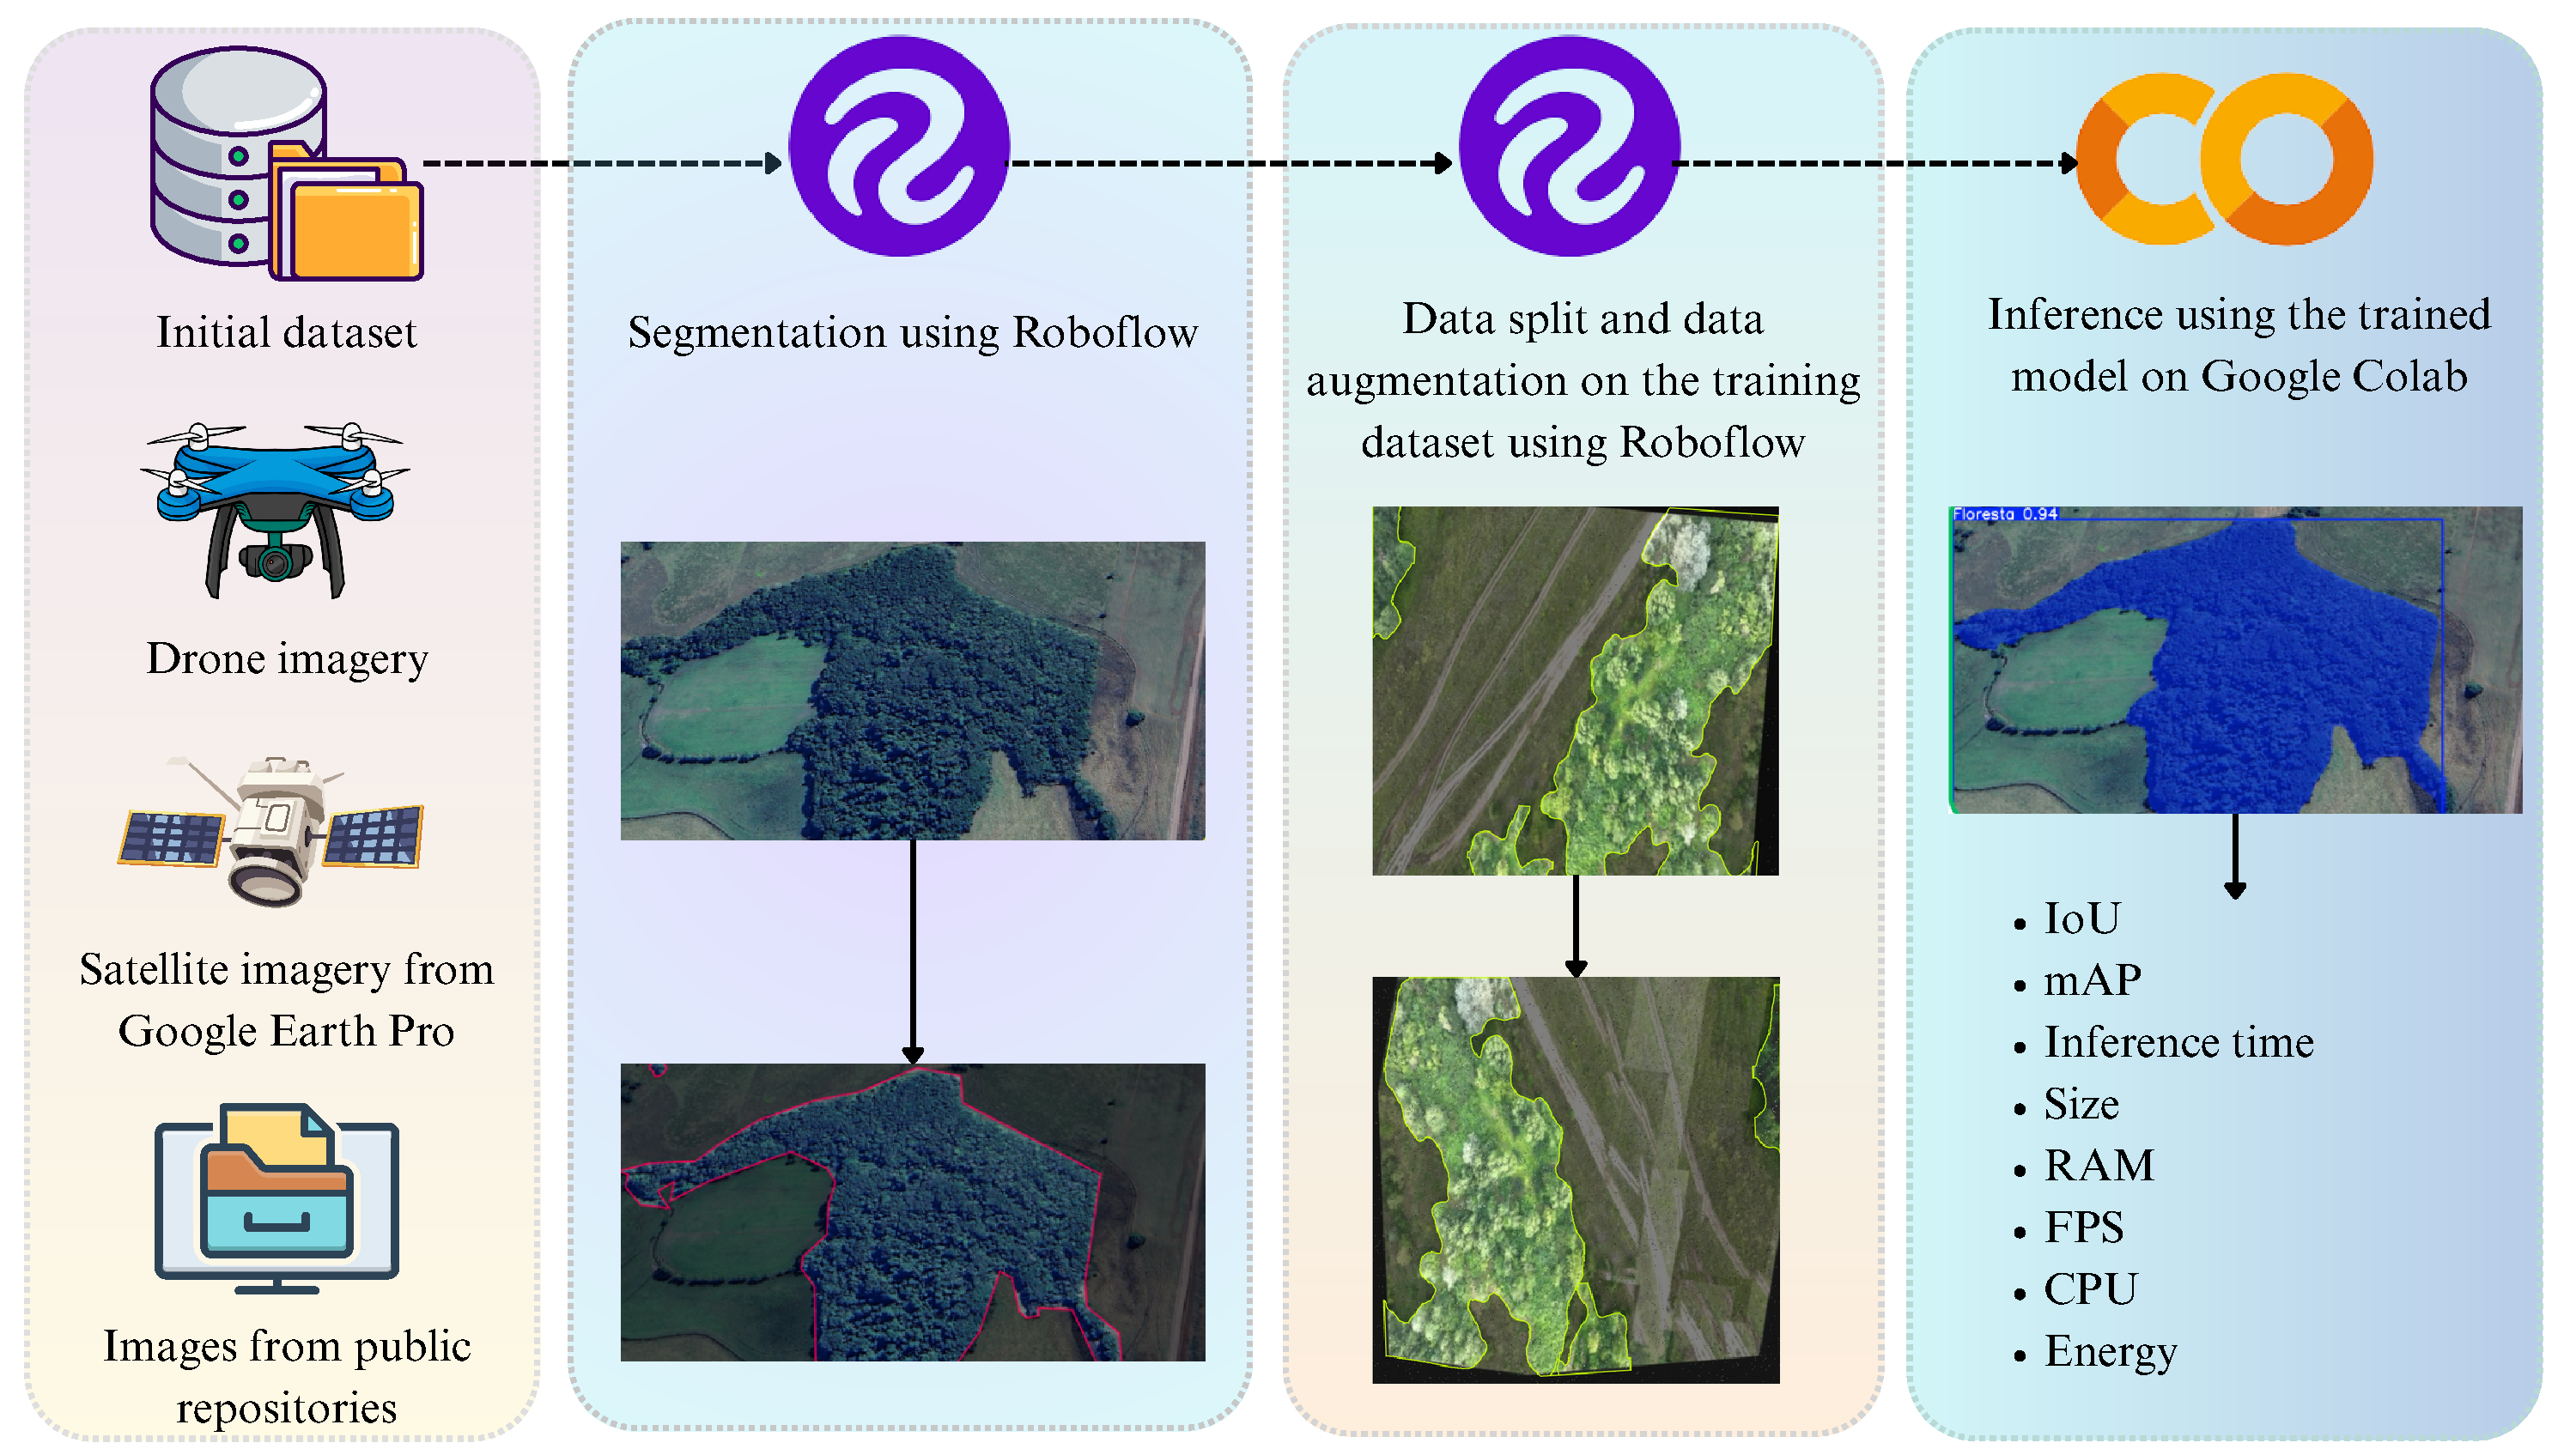
\includegraphics[width=\linewidth]{Figuras/Imagem4.pdf}
    \caption{\small{Overview of the DeforTrack dataset construction and evaluation pipeline.}}
    \label{f1}
\end{figure*}
% Figura 01 %%%%%%%%%%%%%%%%%%%%%%%%%%%%%%%%%%%%%%%%%%%%%%

\textcolor{red}{The remainder of this paper is organized as follows. Section~\ref{sec:dataset} describes the DeforTrack dataset, including data acquisition, annotation methodology, augmentation strategy, and dataset characterization. Section~\ref{sec:evaluation} presents the evaluated deep-learning semantic segmentation models, the training configuration, the proposed forest-area estimation algorithm, and the performance metrics. Section~\ref{sec:results} reports the experimental results, including quantitative benchmarking, external cross-dataset evaluation, qualitative segmentation analysis, and a discussion of the dataset limitations and generalization considerations. Finally, Section~\ref{sec:conclusions} concludes the paper and outlines future research directions.}

\section{Dataset Implementation}
\label{sec:dataset}

This section outlines the processes involved in data acquisition, annotation, augmentation, and organization for the development of the dataset, as illustrated in Fig.~\ref{f1}.

\subsection{Data Collection}

\textcolor{red}{The released dataset comprises RGB images resized to $640 \times 640$ pixels; this value denotes image dimensions, not ground sampling distance (GSD). Images were collected from three main sources: drone-based aerial surveys, imagery accessed through the Google Earth Engine (GEE) platform~\cite{velastegui2023google}, and publicly available environmental image repositories. The final export does not preserve the GEE collection identifiers or a consistent native GSD, so GEE is reported as the access platform rather than as an image sensor. From GEE, we selected regions across Brazil with visible evidence of environmental degradation, such as deforestation scars, forest fragmentation, exposed soil, and transitions between forested and non-forested areas. A total of $400$ images were collected through this procedure. We acquired drone-based imagery through planned UAV missions over forested and partially deforested areas in southeastern Brazil. UAVs were equipped with RGB cameras and operated at altitudes ranging from $800$ to $1,200$ meters. Because camera calibration and flight-level metadata were not preserved in the export, a defensible UAV GSD cannot be reconstructed retrospectively. This process yielded $350$ images.}

Additionally, $5,344$ images were sourced from publicly available environmental monitoring repositories containing aerial and remote-sensing scenes of forested areas, vegetation cover, exposed soil, agricultural surroundings, and forest/non-forest transitions. These external images were included to increase the visual variability of the dataset, covering differences in vegetation structure, canopy density, terrain characteristics, illumination conditions, image acquisition perspective, and non-forest background patterns. These three sources contributed to an initial acquisition pool of $6,094$ images capturing diverse forest structures, vegetation densities, terrain types, and anthropogenic disturbances. \textcolor{red}{The released Roboflow export represents 6,074 source images; therefore, 20 images from the acquisition pool did not enter the released train, validation, or test partitions after annotation and export curation. This distinction between the acquisition pool and the released source-image count reconciles the dataset totals reported below.} Overall, DeforTrack combines drone-based imagery, satellite imagery, and publicly available environmental images to provide a heterogeneous set of forest and non-forest scenes for training and evaluating high-resolution segmentation models under different visual conditions.

\begin{table}[t]
\centering
\caption{Inter-annotator agreement on the validation subset ($n=248$ images).}
\label{tab:interannotator}
\resizebox{\linewidth}{!}{%
\begin{tabular}{|l|c|c|c|c|}
\hline
\textbf{Annotator pair} & \textbf{IoU [\%]} & \textbf{Dice/F1 [\%]} & \textbf{Precision [\%]} & \textbf{Kappa} \\
\hline
Annotator 1 $\times$ Annotator 2 & $71.54 \pm 19.75$ & $81.47 \pm 17.30$ & $81.63 \pm 19.38$ & $0.701 \pm 0.206$ \\ \hline
Annotator 1 $\times$ Annotator 3 & $74.37 \pm 18.36$ & $83.77 \pm 14.80$ & $81.89 \pm 16.68$ & $0.723 \pm 0.206$ \\ \hline
Annotator 2 $\times$ Annotator 3 & $77.73 \pm 20.20$ & $85.49 \pm 17.83$ & $85.97 \pm 14.37$ & $0.759 \pm 0.231$ \\ \hline
\textbf{Mean} & $\mathbf{74.55 \pm 19.44}$ & $\mathbf{83.58 \pm 16.64}$ & $\mathbf{83.17 \pm 16.81}$ & $\mathbf{0.727 \pm 0.216}$ \\ \hline
\end{tabular}%
}
\end{table}

\subsection{Annotation Process}

All images were manually annotated using polygon-based pixel-level masks on the Roboflow platform~\cite{roboflow2026defortrack}, following a binary forest/non-forest labeling protocol. \textcolor{red}{To assess the reliability of the manual annotation process, we conducted an inter-annotator agreement study on a subset of $n=248$ images selected from the validation data after matching the original filenames across annotators.} This subset was independently annotated by three annotators, and the resulting polygon masks were rasterized to a common $640 \times 640$ canvas to enable pixel-wise comparison. For each pair of annotators, we computed the Intersection over Union (IoU), Dice/F1 coefficient~\cite{dice1945measures}, precision, and pixel-level Cohen's Kappa coefficient~\cite{wan2015kappa}, using one annotator as reference and the other as the compared mask. IoU, Dice/F1, precision, and Kappa are reported as \textit{mean} $\pm$ \textit{standard deviation} over the $n=248$ image-level values, and the $95~\%$ confidence interval for the mean IoU was additionally estimated. Table~\ref{tab:interannotator} summarizes the results.
 
The mean pairwise IoU across the three annotator pairs was $74.55 \pm 19.44~\%$, with a mean Dice/F1 of $83.58 \pm 16.64~\%$ and a mean per-image Kappa of $0.727 \pm 0.216$. According to the Landis and Koch scale~\cite{landis1977}, Kappa values between $0.61$ and $0.80$ indicate good agreement, and the mean values for all three annotator pairs fall within this range, although a subset of images with extreme forest-cover ratios ($\approx 0~\%$ or $\approx 100~\%$) yielded lower or occasionally negative per-image Kappa values, since the coefficient is highly sensitive to class imbalance at the single-image level. We additionally computed a two-of-three majority-vote consensus mask for each image and measured each annotator's IoU against this consensus, obtaining $82.75~\%$, $86.67~\%$, and $89.72~\%$ for Annotator 1, Annotator 2, and Annotator 3, respectively. These results demonstrate a good level of agreement among annotators, consistent with the inherent ambiguity of forest/non-forest boundaries in fragmented or transitional landscapes, as discussed in Subsection~\ref{sec:limitations}. This quantitative assessment provides an empirical estimate of labeling quality and annotation uncertainty for the DeforTrack dataset.
 
\subsection{Data Augmentation and Availability}
\label{sec:data_augmentation}

\textcolor{red}{We applied data augmentation techniques only to the annotated training partition, resulting in a final exported dataset with $14,648$ images, including original and augmented samples. The Roboflow output count was configured as three exported samples in total per training example: one original sample and two augmented derivatives. The 12,861 exported training images therefore represent 4,287 source training images. Together with 895 validation and 892 held-out test images, the released partitions represent 6,074 source images in total. The augmentation pipeline included horizontal and vertical flipping, random cropping with $0~\%$ minimum zoom and $20~\%$ maximum zoom, affine shearing of up to $\pm 13^{\circ}$ in both horizontal and vertical directions, brightness adjustment between $-22~\%$ and $+22~\%$, Gaussian blur of up to $3.7$ pixels, and noise injection affecting up to $1.56~\%$ of pixels. These transformations emulate variability associated with illumination, acquisition conditions, and sensor noise. Roboflow performed the data split before augmentation, reducing the risk that augmented derivatives of one original image were assigned to different subsets. As a result, DeforTrack contains $12,861$ training images ($88~\%$), $895$ validation images ($6~\%$), and $892$ held-out final test images ($6~\%$). The validation partition was used for model selection, whereas every result reported in Tables~\ref{tab:segmentation_metrics} and~\ref{tab:computational_metrics} was recomputed on the same 892-image final test partition.}

\textcolor{red}{Although the split was performed before data augmentation, image-level partitioning alone does not guarantee visual, spatial, or temporal independence. We therefore complemented the filename inspection with an exhaustive cross-split visual-similarity audit inspired by the dataset-analysis workflow supported by fastdup~\cite{fastdup2026}. Each of the 14,648 images was represented by the normalized 512-dimensional penultimate-layer embedding of an ImageNet-pretrained ResNet-18~\cite{he2016deep}, and cosine similarity was computed for every train--validation, train--test, and validation--test pair. Validation and test images were used as queries against the training partition. We additionally compared SHA-256 hashes to distinguish byte-identical files from perceptually similar images.}

\begin{table}[ht]
\color{red}
\centering
\caption{Cross-split visual-similarity audit. Counts at 0.98 and 0.99 indicate query images whose nearest cross-split neighbor reached at least the specified cosine similarity.}
\label{tab:split_similarity}
\resizebox{\linewidth}{!}{%
\begin{tabular}{|l|c|c|c|c|c|c|}
\hline
\textbf{Query $\rightarrow$ reference} & \textbf{Queries} & \textbf{Mean nearest} & \textbf{P99 nearest} & \textbf{Maximum} & \textbf{$\geq 0.98$} & \textbf{$\geq 0.99$} \\ \hline
Validation $\rightarrow$ training & 895 & 0.9555 & 0.9882 & 0.9915 & 59 & 4 \\ \hline
Test $\rightarrow$ training & 892 & 0.9494 & 0.9875 & 0.9931 & 45 & 5 \\ \hline
Validation $\rightarrow$ test & 895 & 0.9091 & 0.9764 & 0.9833 & 3 & 0 \\ \hline
\end{tabular}%
}
\end{table}

\textcolor{red}{No byte-identical cross-split image was found by SHA-256. Nevertheless, 59 validation images ($6.59~\%$) and 45 test images ($5.04~\%$) had a training neighbor with cosine similarity of at least 0.98; four and five images, respectively, reached at least 0.99. Manual inspection of the highest-scoring pairs confirmed repeated scenes, strongly overlapping crops, or adjacent video frames across partitions. The earlier filename normalization also identified 586 names potentially associated with more than one subset, but the embedding analysis provides stronger visual evidence than filenames alone. These findings show that the split prevents exact binary duplication but does not eliminate scene-level visual overlap. Consequently, the reported test performance may be optimistic relative to a strictly source-, campaign-, region-, or time-separated evaluation. The complete nearest-neighbor table, top cross-split pairs, embeddings, summary statistics, and visual contact sheet are publicly provided under \texttt{results/split\_similarity/}.}

\subsection{Dataset Diversity Statistics}

Table~\ref{tab:forest_ratio_statistics} reports the forest-cover ratio for each annotated mask, quantifying the internal diversity of DeforTrack. The forest-cover ratio is defined as the number of pixels labeled as forest divided by the total number of pixels in the image. Across the $14,648$ images, the mean forest-cover ratio was $42.71~\%$, with a standard deviation of $26.82~\%$. The values ranged from $0.00~\%$ to $99.99~\%$, indicating that the dataset includes images with very low, intermediate, and nearly complete forest coverage. This distribution provides quantitative evidence of the diversity of forest density and annotation granularity across the dataset.

\begin{table}[t]
\centering
\caption{Quantitative statistics of forest-cover distribution in DeforTrack.}
\label{tab:forest_ratio_statistics}
\begin{tabular}{|l|c|}
\hline
\textbf{Metric} & \textbf{Value} \\
\hline
Total images after augmentation & $14,648$ \\
Mean forest-cover ratio & $42.71~\%$ \\
Standard deviation & $26.82~\%$ \\
Minimum forest-cover ratio & $0.00~\%$ \\
Maximum forest-cover ratio & $99.99~\%$ \\
Images with $0$--$25~\%$ forest cover & $4,903$ \\
Images with $25$--$50~\%$ forest cover & $4,053$ \\
Images with $50$--$75~\%$ forest cover & $3,288$ \\
Images with $75$--$100~\%$ forest cover & $2,404$ \\
\hline
\end{tabular}
\end{table}

% Figura 02 %%%%%%%%%%%%%%%%%%%%%%%%%%%%%%%%%%%
\begin{figure*}[!ht]
    \centering
    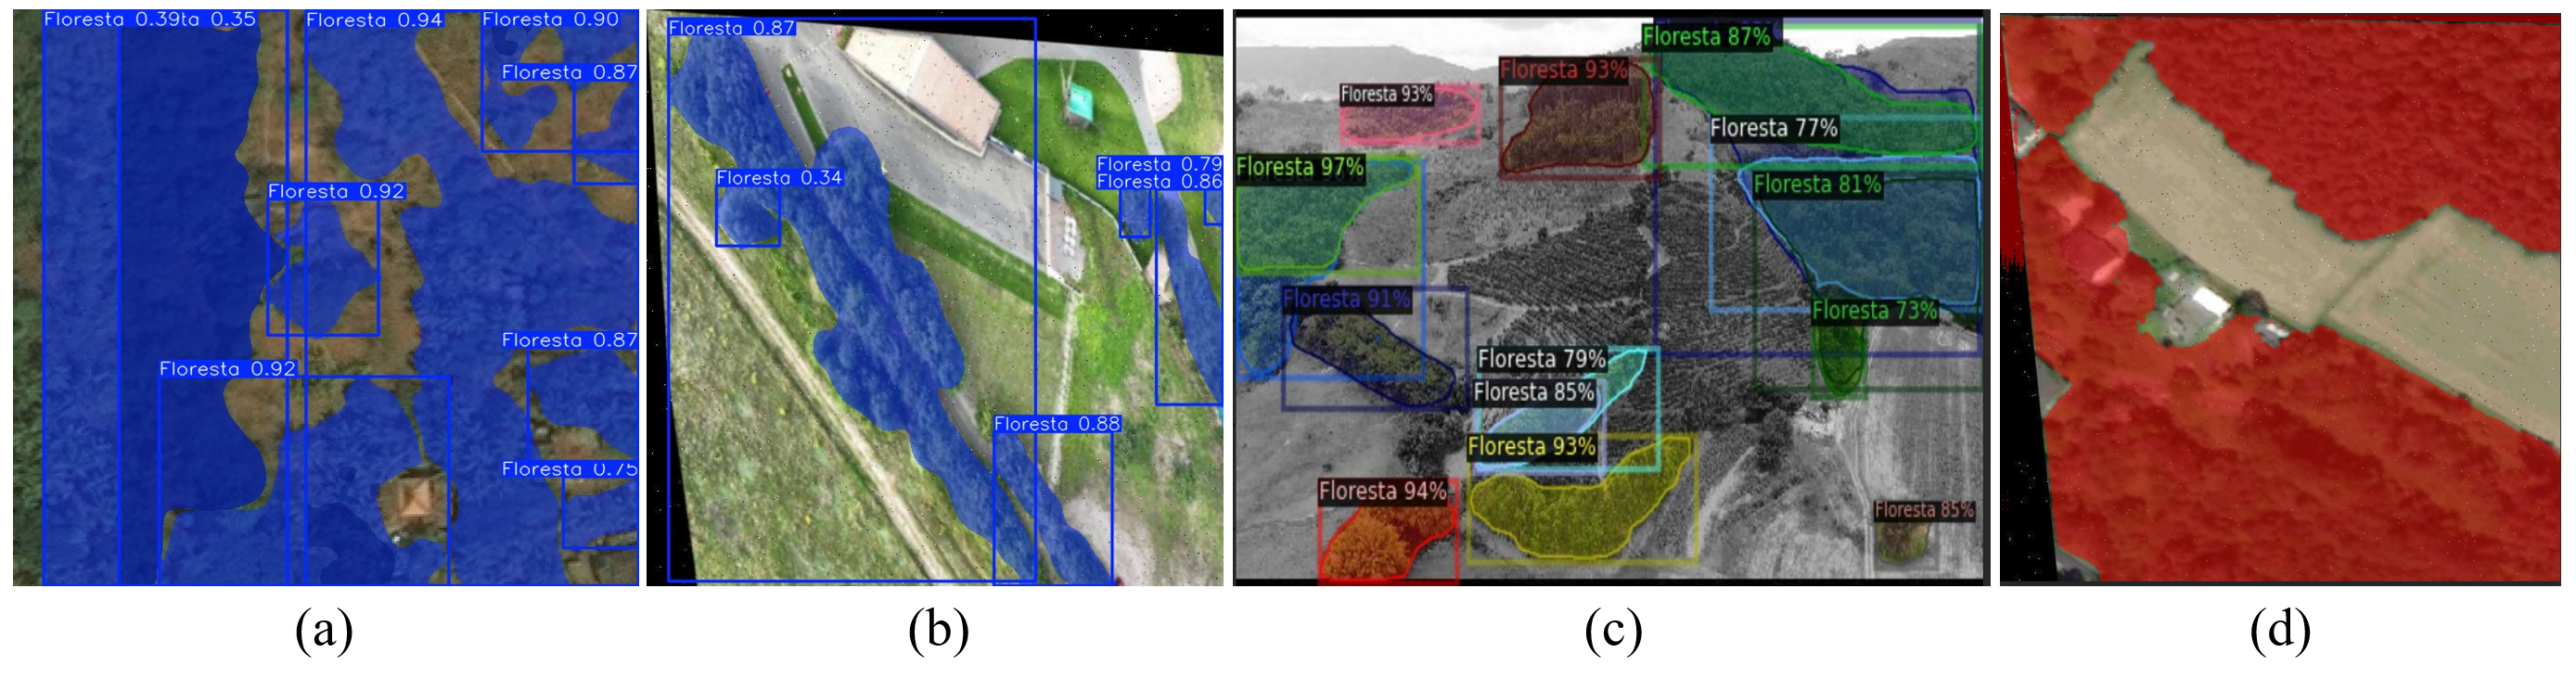
\includegraphics[width=\linewidth]{Figuras/Imagem2.png}
    \caption{\small{Segmented mask outputs from models (a) YOLOv8x, (b) YOLOv11s, (c) Mask R-CNN R101 C4 3x, and (d) U-Net.}}
    \label{f2}
\end{figure*}
% Figura 02 %%%%%%%%%%%%%%%%%%%%%%%%%%%%%%%%%%%


\section{Deep-learning Semantic Segmentation Models Evaluation}
\label{sec:evaluation}

We conducted a comprehensive evaluation of state-of-the-art semantic segmentation models widely used in remote sensing and computer vision to assess the DeforTrack dataset. This section describes the training setup, segmentation pipeline, forest area estimation methodology, and performance metrics used for model benchmarking.

\subsection{Deep-learning models and training setup}

\textcolor{red}{The evaluation encompassed multiple deep learning architectures selected for their relevance to environmental monitoring and their distinct accuracy--complexity profiles. The tested models include U-Net, Mask R-CNN (Region-based Convolutional Neural Network) via Detectron2, and two versions of the YOLO (You Only Look Once) family (YOLOv8 and YOLOv11), with the evaluation code publicly available\footnote{\url{https://github.com/alvarosamp/DeforTrack}}.}
\textcolor{red}{For YOLO-based models, we considered five variants per version: nano, small, medium, large, and extra-large, capturing a range of trade-offs between computational load and accuracy. Similarly, multiple Mask R-CNN variants were evaluated, differing in backbone depth (ResNet-50 vs. ResNet-101) and head configuration (C4, DC5, and FPN). The U-Net model was included as a semantic-segmentation baseline due to its prevalence in geospatial segmentation tasks and its interpretable architecture. Model training was performed in Google Colab using Python 3 and an NVIDIA T4 GPU. After training, all final segmentation evaluations and computational profiles reported in this work were executed on the same local workstation running 64-bit Windows 11 Education, with an Intel Core i9-13900HX processor (24 physical cores and 32 logical processors), 16 GB of system RAM, and an NVIDIA GeForce RTX 4060 Laptop GPU with 8 GB of VRAM (driver 610.62), using Python 3.11.9, PyTorch 2.8.0 with CUDA 12.9, Ultralytics 8.4.96, Detectron2 0.6, Keras 3.15.0, and OpenCV 5.0.0. Thus, latency, throughput, resource-use, and energy results are measurements from the local RTX 4060 Laptop GPU workstation, not from the T4 used for training or from an embedded platform.}

\textcolor{red}{During final-test inference, YOLO and Mask R-CNN processed $640\times640$ inputs with confidence thresholds of 0.25 and 0.30, respectively. The Mask R-CNN export metadata contains the synonymous foreground labels ``Forest'' and ``Floresta''; predictions from these two labels were mapped to one binary forest class before region- and boundary-metric computation and before binary COCO-style mask AP evaluation. U-Net processed RGB inputs resized to $256\times256$ and binarized its probability map at 0.50. The corresponding reference polygons were rasterized at each model's evaluation resolution, and predictions were restored to the reference dimensions whenever necessary.}

\textcolor{red}{The operating-system build was 10.0.26200, and the GPU reported 8,188~MiB of dedicated memory. Additional dependencies included NumPy 2.4.4, \texttt{psutil} 7.2.2, and NVIDIA Management Library bindings 13.610.43. The profiling script did not explicitly enable mixed precision. GPU power-limit, clock-frequency, thermal, and operating-system power-profile settings were not logged by the profiling procedure. Consequently, fixed operating conditions cannot be established retrospectively. Laptop power management, cooling, and background workloads may contribute to measurement variability. Warm-up and repeated measurements reduce transient effects but do not eliminate these sources of variability.}

\subsection{Pixel-wise Mask Fusion for Forest Area Estimation}
\label{subsec:algorithm}

\textcolor{red}{We applied a post-processing algorithm that aggregates the same-class instance masks produced for one image by one model inference. Outputs from different model architectures are not fused. For an instance-based prediction, let $M_k \in \{0,1\}^{m \times n}$ denote the $k$th accepted forest-instance mask, where a value of 1 indicates forest at a given pixel coordinate. A semantic model such as U-Net already produces one binary mask, for which the aggregation is the identity operation. Figure~\ref{f2} shows representative final semantic masks for YOLOv8x, YOLOv11s, Mask R-CNN, and U-Net. For an instance-based output, the final semantic mask $M_f$ is computed via a pixel-wise Boolean OR across its $k$ forest-instance masks.}

\begin{equation} \label{eq1}
    M_f = M^1 \lor M^2 \lor \cdots \lor M^k,
\end{equation}

where $\lor$ denotes the Boolean OR operator. Each element $M_{ij}^f$ of the
final mask is given by

\begin{equation}
M_{ij}^f = M_{ij}^1 \lor M_{ij}^2 \lor \cdots \lor M_{ij}^k.
\end{equation}

\textcolor{red}{The resulting final mask $M_f$ is then used to compute the percentage of forest cover $A_f$ in the image, given by:}

{\color{red}
\begin{equation}
    A_f = 100 \times \frac{1}{m\times n}\sum_{i=1}^{m} \sum_{j=1}^{n} M_{ij}^f.
\end{equation}
}

This method provides a simple and efficient estimate of forest-cover percentage
from the segmentation outputs. In this work, the method was evaluated as a
post-processing step under the same computational setup used for model
benchmarking.

\textcolor{red}{The union operation was adopted because each predicted instance mask represents
a candidate forest region. Therefore, a pixel is classified as forest if it is
included in at least one predicted forest mask. This strategy avoids discarding
valid forest pixels when multiple masks partially overlap or when a forest
region is split into more than one predicted instance. In contrast, an
intersection-based rule would be overly restrictive, since only pixels shared by
all masks would be retained. A weighted average was not adopted because it would
require calibrated and mutually comparable pixel-level confidence values, as well as an additional threshold selected on validation data. The Boolean OR therefore implements the geometrically correct union of same-class forest instances without introducing an unvalidated fusion parameter.}

\textcolor{red}{We empirically compared these alternatives using the Mask R-CNN ResNet-101 FPN 3x model, whose instance outputs make all three fusion rules applicable. Candidate instances were first filtered with the same confidence threshold of 0.30 used in the main evaluation. For weighted fusion, each binary instance mask was weighted by its confidence score and normalized by the sum of scores. Its binarization threshold was selected exclusively on the 895-image validation partition from values between 0.05 and 0.95 in increments of 0.05; the selected threshold of 0.05 was then frozen and applied to the 892-image final test partition. Table~\ref{tab:fusion_ablation} reports macro-averaged test results. OR achieved $77.92~\%$ IoU and $85.88~\%$ Dice/F1, whereas AND achieved only $13.78~\%$ IoU and $14.77~\%$ Dice/F1 because the intersection retains only pixels shared by every predicted instance, which is unsuitable when separate masks represent spatially disjoint forest regions. The calibrated weighted mean also achieved $77.92~\%$ IoU and $85.88~\%$ Dice/F1. It differed from OR in only 9 of the 892 test images, with a mean IoU difference of $0.0032$ percentage points. This negligible difference indicates that weighting the already thresholded instance masks did not provide a practically meaningful improvement. Because weighted fusion introduced an additional validation-dependent threshold while OR directly preserved every accepted forest instance, OR was retained as the final fusion rule. This conclusion is restricted to the evaluated Mask R-CNN variant and protocol and should not be interpreted as universal superiority of OR over all possible fusion methods.}

\begin{table}[t]
\color{red}
\centering
\caption{Ablation of instance-mask fusion rules on the 892-image final test partition using Mask R-CNN ResNet-101 FPN 3x. OR and weighted-mean values coincide at two-decimal precision; their per-image predictions differed in 9 cases, with a mean IoU difference of 0.0032 percentage points.}
\label{tab:fusion_ablation}
\resizebox{\linewidth}{!}{%
\begin{tabular}{|l|c|c|c|c|c|}
\hline
\textbf{Fusion} & \textbf{IoU [\%]} & \textbf{Dice/F1 [\%]} & \textbf{Precision [\%]} & \textbf{Recall [\%]} & \textbf{Pixel Acc. [\%]} \\ \hline
OR & 77.92 & 85.88 & 83.45 & 91.89 & 90.16 \\ \hline
AND & 13.78 & 14.77 & 18.98 & 14.34 & 63.91 \\ \hline
Weighted mean & \textbf{77.92} & \textbf{85.88} & \textbf{83.45} & 91.89 & \textbf{90.16} \\ \hline
\end{tabular}%
}
\end{table}



\subsection{Evaluation Metrics}

Model performance was quantitatively assessed using both accuracy-oriented and resource-efficiency metrics:
\begin{itemize}
    \item \textbf{Intersection over Union (IoU):} Measures the overlap between the predicted mask $M_p$ and the ground truth mask $M_t$. It is defined as:
    \[
    \text{IoU} = \frac{\sum_{i=1}^{m} \sum_{j=1}^{n} (M_{p_{ij}} \land M_{t_{ij}})}{\sum_{i=1}^{m} \sum_{j=1}^{n} (M_{p_{ij}} \lor M_{t_{ij}})},
    \]
    where $\land$ and $\lor$ represent the Boolean AND and OR operations, respectively. The mask used to calculate the IoU is the $M^f$ defined in (1).
    \item \textcolor{red}{\textbf{Dice/F1:} Measures region overlap as $2TP/(2TP+FP+FN)$, where $TP$, $FP$, and $FN$ denote forest-pixel true positives, false positives, and false negatives.}
    \item \textcolor{red}{\textbf{Precision, Recall, and Pixel Accuracy:} Precision is $TP/(TP+FP)$, recall is $TP/(TP+FN)$, and pixel accuracy is $(TP+TN)/(TP+TN+FP+FN)$, with $TN$ denoting correctly classified non-forest pixels.}
    \item \textcolor{red}{\textbf{Boundary IoU and Boundary F1:} Boundaries were extracted from the binary prediction and reference masks by morphological erosion with a three-pixel thickness. Boundary IoU measures the intersection over union of the resulting boundary bands. Boundary F1 is the harmonic mean of boundary precision and recall, allowing a three-pixel spatial tolerance through morphological dilation.}
    \item \textbf{Mean Average Precision (mAP):} Evaluates the overall detection and localization performance by averaging the precision across multiple IoU thresholds.
    \item \textbf{Inference Time and FPS:} Represent the average time (in seconds) required to segment a single image and the effective throughput in frames per second, respectively.
    \item \textcolor{red}{\textbf{Computational Resource Metrics:} Include peak process RAM, normalized process CPU utilization, and GPU energy per image during inference. These measurements provide a controlled comparison on the specified workstation and do not represent embedded-device performance.}
    %They allow for assessing the deployability of models on real-time and embedded systems.
\end{itemize}

\textcolor{red}{The evaluations were performed on the same held-out final test subset of 892 images for every YOLO, Mask R-CNN, and U-Net variant. For instance-based architectures, mAP@50 and mAP@50--95 were computed from individual predicted instances, with the latter averaging IoU thresholds from 0.50 to 0.95 in steps of 0.05. Because the U-Net checkpoint produces one semantic binary mask without instance confidence scores, instance-level mAP is not applicable and is reported as ``--'' rather than being inferred from pixel-level metrics.}

\textcolor{red}{For the pixel-level metrics, all predicted forest instances from one image were merged by the union in (\ref{eq1}), and the resulting binary semantic mask was compared with the rasterized reference mask. IoU, Dice/F1, precision, recall, Boundary IoU, Boundary F1, and pixel accuracy were first computed independently for each image and then macro-averaged over the 892 test images. This preserves equal image weighting and avoids allowing images with more forest pixels to dominate the aggregate.}
%Regarding the mAP, we set an IoU threshold of 0.5 and a second metric with it varying between 0.5 and 0.95.
\textcolor{red}{Computational profiling used batch size 1, one complete unmeasured warm-up pass over the 892-image final test set to stabilize model execution and GPU clocks, and three subsequent complete measured repetitions, totaling 2,676 measured inferences per checkpoint. Before the warm-up and measurement stages, the complete test set was read once to warm the operating-system file cache, and each decoded image was immediately released, preventing disk-cache order effects without retaining the decoded dataset in process RAM. Reported latency is the mean end-to-end time per image for image decoding, model-specific preprocessing, GPU inference, explicit GPU synchronization, and prediction return; FPS is its reciprocal. Peak resident set size (RAM) and process CPU use were monitored with \texttt{psutil}. CPU utilization was divided by the 32 logical processors and is consequently reported on a normalized $0$--$100~\%$ system scale. GPU board power was sampled through the NVIDIA Management Library (NVML) during the measured loop. GPU energy was obtained by trapezoidal integration of power over elapsed time and divided by 2,676, so Table~\ref{tab:computational_metrics} reports joules per image rather than total energy, batch energy, or whole-system energy.}

\textcolor{red}{To provide uncertainty estimates and improve repeatability analysis, we computed confidence intervals for the main image-level metrics. For each metric, the mean value was computed over the 892 final test images, and the $95~\%$ confidence interval was estimated as:}
\begin{equation}
CI_{95\%} = \bar{x} \pm 1.96 \cdot \frac{s}{\sqrt{n}},
\end{equation}
where $\bar{x}$ is the sample mean, $s$ is the standard deviation across test images, and $n$ is the number of evaluated images. This analysis provides an estimate of the uncertainty associated with the reported average performance and complements the single-point values reported in the comparison tables.

\section{Results and Discussion}
\label{sec:results}

\textcolor{red}{This section presents the standardized performance analysis of all trained checkpoints. Tables~\ref{tab:segmentation_metrics} and~\ref{tab:computational_metrics} report results obtained on the same 892-image held-out final test set. YOLOv8s achieved the highest region-level segmentation scores overall, with $89.03~\%$ IoU, $93.73~\%$ Dice/F1, and $96.02~\%$ pixel accuracy, as well as the highest recall ($95.18~\%$). YOLOv8l obtained the highest mAP@50 ($92.79~\%$). YOLOv8x reached only $71.57~\%$ IoU despite being the largest YOLOv8 variant. This isolated checkpoint result shows that greater parameter count did not guarantee better mask overlap in the present run, but it should not be interpreted as an architectural limitation without controlled repeated training, seed analysis, and checkpoint diagnostics. Within YOLOv11, the medium variant obtained the highest IoU ($88.78~\%$), while YOLOv11x achieved the strongest boundary performance, with $48.04~\%$ Boundary IoU and $70.22~\%$ Boundary F1. YOLOv11l obtained the highest mAP@50--95 of all evaluated checkpoints ($74.19~\%$). These rankings differ by metric because region overlap, instance detection across thresholds, and boundary localization emphasize different error modes; consequently, no single score is used to claim universal superiority.}

For instance, Figure~\ref{f3}(a--b) displays two images of the same region captured at two different dates. The YOLOv11n model processed these images, and the
resulting segmentation masks were integrated using the proposed pixel-based
algorithm to estimate the percentage of forested area, as described in
Subsection~\ref{subsec:algorithm}. Figures~\ref{f3}(c--d) show the
corresponding outputs with the estimated forest-cover percentages. Based on the
processing defined in~(3), the initial forest coverage was estimated at
$51.78~\%$, while the second image presented $72.92~\%$ of forest coverage.
These results demonstrate the applicability of the proposed method for
quantifying vegetation-cover variation over time.

\begin{table*}[t]
\centering
\color{red}
\caption{Segmentation performance on the same 892-image final test partition of DeforTrack.}
\label{tab:segmentation_metrics}
\resizebox{\textwidth}{!}{%
\begin{tabular}{|c|c|c|c|c|c|c|c|c|c|c|}
\hline
\textbf{Variant} & \textbf{Images} & \textbf{IoU [\%]} & \textcolor{red}{\textbf{mAP@50 [\%]}} & \textcolor{red}{\textbf{mAP@50--95 [\%]}} & \textbf{Dice/F1 [\%]} & \textbf{Boundary IoU [\%]} & \textbf{Boundary F1 [\%]} & \textbf{Pixel Accuracy [\%]} & \textbf{Precision [\%]} & \textbf{Recall [\%]} \\
\hline

\multicolumn{11}{|c|}{\textbf{YOLOv8 Performance}} \\ \hline
YOLOv8x & 892 & 71.57 & 88.83 & 64.10 & 77.75 & 39.37 & 59.10 & 82.19 & 84.47 & 77.01 \\ \hline
YOLOv8l & 892 & 88.02 & \textbf{92.79} & 72.56 & 92.97 & 45.02 & 66.74 & 95.23 & 92.54 & 94.14 \\ \hline
YOLOv8m & 892 & 83.82 & 84.89 & 55.82 & 90.32 & 34.97 & 54.65 & 93.83 & 89.90 & 91.80 \\ \hline
YOLOv8s & 892 & \textbf{89.03} & 92.02 & 71.12 & \textbf{93.73} & 45.10 & 66.58 & \textbf{96.02} & 92.88 & \textbf{95.18} \\ \hline
YOLOv8n & 892 & 86.33 & 91.70 & 68.35 & 91.86 & 40.95 & 62.15 & 94.58 & 91.30 & 93.28 \\ \hline

\multicolumn{11}{|c|}{\textbf{YOLOv11 Performance}} \\ \hline
YOLOv11x & 892 & 88.60 & 92.66 & 74.18 & 93.20 & \textbf{48.04} & \textbf{70.22} & 95.15 & \textbf{93.40} & 94.11 \\ \hline
YOLOv11l & 892 & 88.30 & 92.09 & \textbf{74.19} & 92.88 & 47.53 & 69.72 & 95.03 & 92.87 & 93.98 \\ \hline
YOLOv11m & 892 & 88.78 & 92.28 & 73.06 & 93.36 & 47.96 & 70.02 & 95.49 & 93.12 & 94.52 \\ \hline
YOLOv11s & 892 & 87.88 & 92.46 & 72.03 & 92.77 & 45.36 & 67.18 & 95.05 & 92.62 & 94.00 \\ \hline
YOLOv11n & 892 & 87.19 & 91.57 & 67.91 & 92.51 & 41.06 & 62.25 & 95.10 & 91.69 & 94.05 \\ \hline

\multicolumn{11}{|c|}{\textbf{Mask R-CNN Performance}} \\ \hline
ResNet-101 FPN 3x & 892 & 77.92 & 68.84 & 41.11 & 85.88 & 25.58 & 42.02 & 90.16 & 83.45 & 91.89 \\ \hline
ResNet-101 C4 3x & 892 & 77.48 & 61.33 & 39.15 & 85.59 & 23.88 & 39.46 & 90.24 & 85.24 & 89.18 \\ \hline
ResNet-101 DC5 3x & 892 & 73.05 & 56.22 & 31.80 & 81.44 & 23.09 & 38.46 & 85.96 & 80.47 & 89.36 \\ \hline
ResNet-50 C4 3x & 892 & 75.92 & 56.58 & 34.31 & 84.82 & 22.90 & 38.02 & 89.74 & 84.44 & 88.26 \\ \hline
ResNet-50 C4 1x & 892 & 75.59 & 56.03 & 33.88 & 84.37 & 21.54 & 36.12 & 89.29 & 83.24 & 89.13 \\ \hline
ResNet-50 DC5 1x & 892 & 77.66 & 59.02 & 35.09 & 85.91 & 25.07 & 41.36 & 90.51 & 85.35 & 89.38 \\ \hline

\multicolumn{11}{|c|}{\textbf{U-Net Performance}} \\ \hline
U-Net & 892 & 49.97 & -- & -- & 61.80 & 20.93 & 34.53 & 72.50 & 70.11 & 68.14 \\ \hline
\end{tabular}%
}
\end{table*}

\begin{table*}[t] \small
\color{red}
\centering
\caption{Standardized computational performance on the same 892-image final test set. Inference time is reported as mean $\pm$ standard deviation across three complete measured repetitions.}
\label{tab:computational_metrics}
\resizebox{\textwidth}{!}{%
\begin{tabular}{|c|c|c|c|c|c|c|c|}
\hline
\textbf{Variant} & \textbf{Images} & \textbf{Size [MB]} & \textbf{Peak process RAM [MB]} & \textbf{Inference [s/image]} & \textbf{FPS} & \textbf{Normalized CPU [\%]} & \textbf{GPU energy [J/image]} \\
\hline

\multicolumn{8}{|c|}{\textbf{YOLOv8 Performance}} \\ \hline
YOLOv8x & 892 & 274.25 & 1527.98 & $0.0493 \pm 0.0004$ & 20.28 & 3.34 & 3.808 \\ \hline
YOLOv8l & 892 & 175.77 & 1499.66 & $0.0325 \pm 0.0002$ & 30.73 & 3.16 & 2.439 \\ \hline
YOLOv8m & 892 & 104.35 & 1483.15 & $0.0223 \pm 0.0002$ & 44.88 & 3.23 & 1.438 \\ \hline
YOLOv8s & 892 & 22.78 & 1383.85 & $0.0131 \pm 0.0001$ & 76.20 & 3.14 & 0.675 \\ \hline
YOLOv8n & 892 & 12.81 & 1357.66 & $\mathbf{0.0120 \pm 0.0001}$ & \textbf{83.39} & 3.14 & \textbf{0.263} \\ \hline

\multicolumn{8}{|c|}{\textbf{YOLOv11 Performance}} \\ \hline
YOLOv11x & 892 & 119.01 & 1531.60 & $0.0476 \pm 0.0003$ & 21.03 & 3.27 & 3.722 \\ \hline
YOLOv11l & 892 & 53.28 & 1437.52 & $0.0290 \pm 0.0009$ & 34.49 & 3.18 & 1.839 \\ \hline
YOLOv11m & 892 & 43.09 & 1433.00 & $0.0226 \pm 0.0003$ & 44.30 & 3.21 & 1.471 \\ \hline
YOLOv11s & 892 & 19.59 & 1395.61 & $0.0164 \pm 0.0002$ & 61.07 & \textbf{3.10} & 0.719 \\ \hline
YOLOv11n & 892 & \textbf{5.75} & 1337.91 & $0.0156 \pm 0.0004$ & 64.00 & 3.15 & 0.279 \\ \hline

\multicolumn{8}{|c|}{\textbf{Mask R-CNN Performance}} \\ \hline
ResNet-101 FPN 3x & 892 & 479.84 & 1949.74 & $0.0483 \pm 0.0009$ & 20.72 & 3.21 & 2.833 \\ \hline
ResNet-101 C4 3x & 892 & 412.46 & 1872.13 & $0.0389 \pm 0.0009$ & 25.73 & 3.18 & 2.325 \\ \hline
ResNet-101 DC5 3x & 892 & 1456.46 & 3462.20 & $0.0509 \pm 0.0004$ & 19.64 & 3.17 & 3.386 \\ \hline
ResNet-50 C4 3x & 892 & 267.47 & 1767.68 & $0.0310 \pm 0.0002$ & 32.25 & 3.20 & 1.796 \\ \hline
ResNet-50 C4 1x & 892 & 267.47 & 1708.98 & $0.0317 \pm 0.0003$ & 31.52 & 3.23 & 1.811 \\ \hline
ResNet-50 DC5 1x & 892 & 1311.47 & 3337.60 & $0.0425 \pm 0.0006$ & 23.51 & 3.19 & 2.753 \\ \hline

\multicolumn{8}{|c|}{\textbf{U-Net Performance}} \\ \hline
U-Net & 892 & 21.63 & \textbf{985.39} & $0.0154 \pm 0.0002$ & 64.77 & 3.37 & 0.909 \\ \hline

\end{tabular}
}
\end{table*}

\begin{figure}[h]
    \centering
    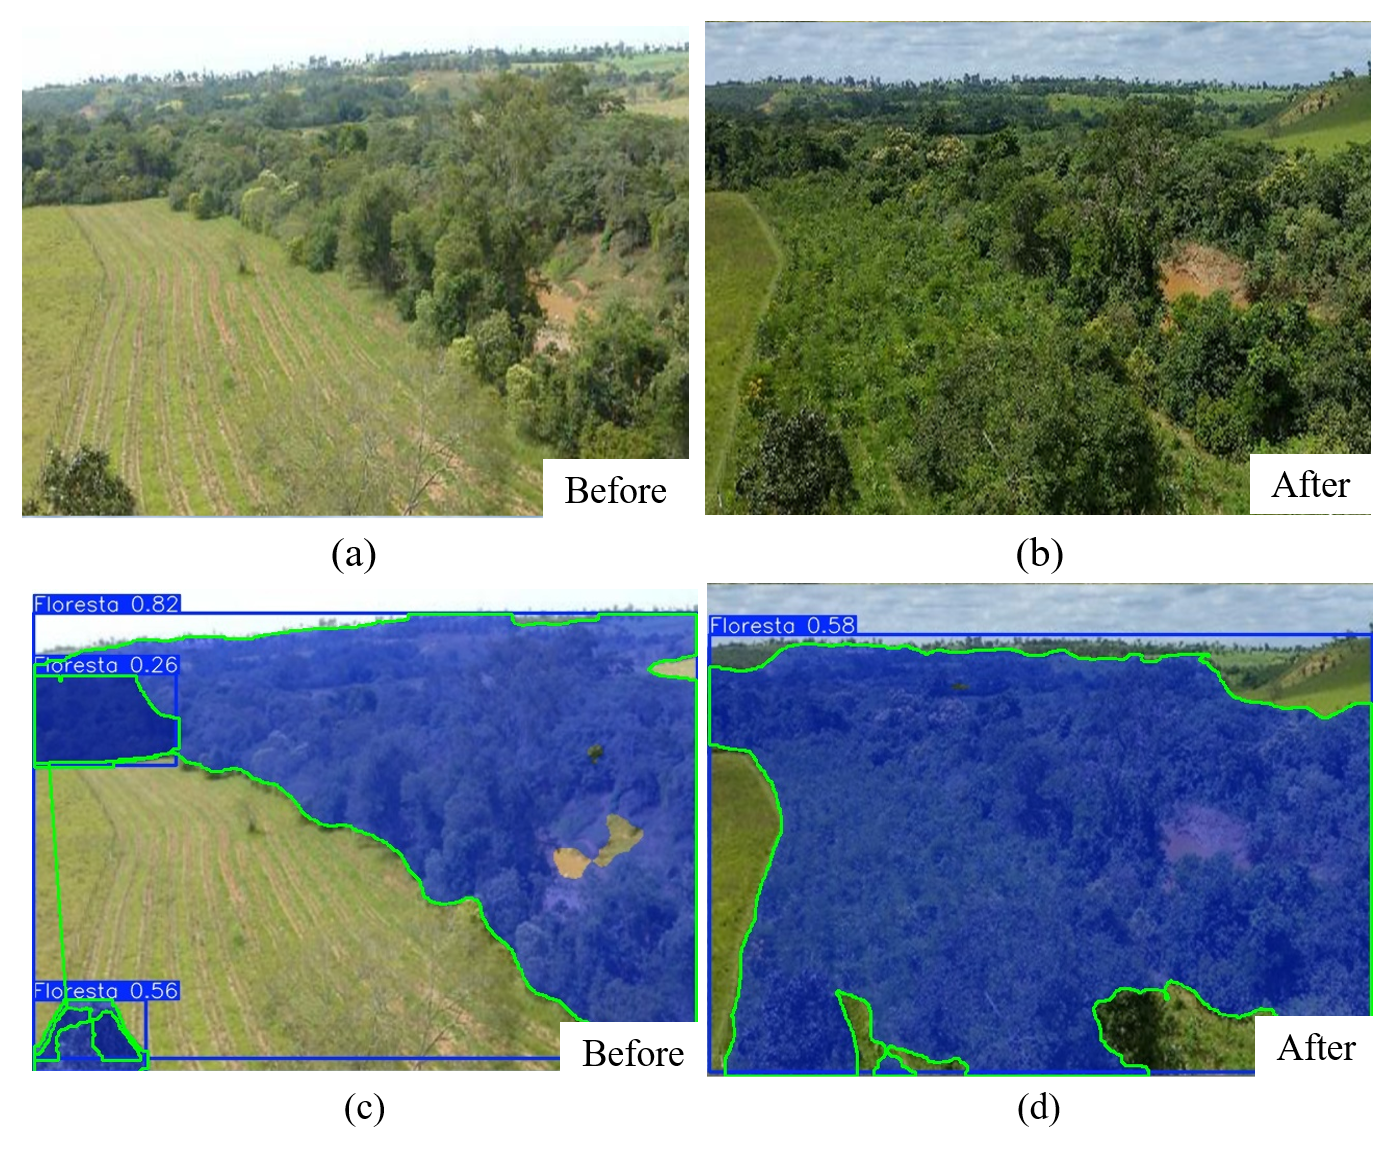
\includegraphics[width=\linewidth]{Figuras/Imagem3.png}
    \caption{\small{Example of vegetation-cover change estimation using the proposed pixel-based algorithm. Images (a) and (b) show the input scenes acquired at two different dates, before and after vegetation change, respectively. Images (c) and (d) show the corresponding segmentation outputs generated by the model and used by the pixel-based algorithm to estimate forest-cover percentage.}}
    \label{f3}
\end{figure}

\textcolor{red}{The per-image uncertainty analysis supports the same ordering while showing the variability within the test set. The $95~\%$ confidence-interval half-width for IoU was $0.74$ percentage points for YOLOv8s, $1.27$ percentage points for Mask R-CNN ResNet-101 FPN 3x, and $1.79$ percentage points for U-Net. Complete per-image values are publicly available in the model-specific files under \texttt{results/internal\_test\_892/}. A structured supplementary table covering all 17 checkpoints and seven pixel-level metrics is provided as \texttt{results/consolidated/internal\_uncertainty\_all\_models.csv}; each row reports the number of test images, mean, standard deviation, 95\% confidence-interval half-width, and lower and upper confidence limits. These public machine-readable files provide the complete uncertainty results without further widening Table~\ref{tab:segmentation_metrics}.}

\textcolor{red}{We additionally performed a sensitivity analysis for the visual overlap identified in Table~\ref{tab:split_similarity}. The 45 final-test images whose nearest training neighbor had cosine similarity greater than or equal to 0.98 were excluded, and all seven per-image segmentation metrics were recomputed on the remaining 847 images without retraining or changing any model threshold. Table~\ref{tab:similarity_filtered} reports representative checkpoints. YOLOv8s changed from $89.029~\%$ to $89.027~\%$ IoU, and the largest absolute IoU change among all 17 checkpoints was 0.441 percentage points. Thus, the high-similarity subset does not explain the principal internal ranking under this threshold. This diagnostic exclusion nevertheless does not create a geographically or temporally independent test set, because source-level provenance is unavailable and visually related samples may remain below the selected similarity threshold. Complete results and the excluded-image manifest are provided under \texttt{results/similarity\_filtered\_test/}.}

\begin{table}[t]
\color{red}
\centering
\caption{Sensitivity analysis after excluding 45 final-test images with a train--test cosine similarity of at least 0.98. Complete results for all 17 checkpoints are provided in the repository.}
\label{tab:similarity_filtered}
\resizebox{\linewidth}{!}{%
\begin{tabular}{|l|c|c|c|c|c|}
\hline
\textbf{Model} & \textbf{$n$} & \textbf{Full IoU [\%]} & \textbf{Filtered IoU [\%]} & \textbf{$\Delta$ IoU [pp]} & \textbf{Filtered Dice/F1 [\%]} \\ \hline
YOLOv8s & 847 & 89.029 & 89.027 & -0.002 & 93.733 \\ \hline
YOLOv11m & 847 & 88.779 & 89.163 & +0.384 & 93.717 \\ \hline
Mask R-CNN R-101 FPN 3x & 847 & 77.920 & 77.549 & -0.370 & 85.631 \\ \hline
U-Net & 847 & 49.969 & 49.643 & -0.326 & 61.458 \\ \hline
\end{tabular}%
}
\end{table}

\textcolor{red}{The inter-annotator mean IoU of $74.55~\%$ in Table~\ref{tab:interannotator} should not be interpreted as a human-performance ceiling directly comparable with the $89.03~\%$ YOLOv8s test IoU. Inter-annotator agreement was measured on a separate 248-image validation subset and quantifies disagreement between independently drawn masks, whereas model performance was measured on the 892-image final test set against its released reference masks. A controlled human--model comparison would require predictions and multiple independent annotations for the same images and reference construction. The similarity-filtered analysis above addresses one potential source of optimism, while the absence of source-, location-, and time-aware grouping remains a separate limitation.}

\textcolor{red}{The standardized results identify different leaders depending on the evaluation criterion. YOLOv8s achieved the highest region-level IoU ($89.03~\%$), Dice/F1 ($93.73~\%$), and pixel accuracy ($96.02~\%$), while maintaining $0.0131 \pm 0.0001$~s/image, 76.20 FPS, and 0.675 GPU J/image. YOLOv11x produced the strongest boundary metrics (Boundary IoU $48.04~\%$ and Boundary F1 $70.22~\%$), but required $0.0476 \pm 0.0003$~s/image and 3.722 GPU J/image. These results show that selecting a model only by region overlap can obscure differences in contour quality and computational cost.}

\textcolor{red}{Among the lightweight variants, YOLOv8n was the fastest and least energy-intensive checkpoint, reaching $0.0120 \pm 0.0001$~s/image, 83.39 FPS, and 0.263 GPU J/image. YOLOv11n had the smallest checkpoint (5.75 MB), but was slower at $0.0156 \pm 0.0004$~s/image and 64.00 FPS. Thus, checkpoint size alone did not determine workstation latency. YOLOv8s retained substantially higher segmentation accuracy than both nano variants while remaining close to their throughput, making it the strongest accuracy--efficiency compromise in this experiment. Mask R-CNN remained competitive in region segmentation but incurred higher resource use. ResNet-101 FPN 3x was the best Mask R-CNN variant by IoU ($77.92~\%$), with $0.0483 \pm 0.0009$~s/image, 20.72 FPS, 1949.74 MB peak process RAM, and 2.833 GPU J/image. ResNet-50 C4 3x was the fastest Mask R-CNN variant at $0.0310 \pm 0.0002$~s/image and 32.25 FPS, but its IoU was lower at $75.92~\%$. U-Net had the lowest peak process RAM (985.39 MB) and reached 64.77 FPS; its IoU ($49.97~\%$) and Boundary IoU ($20.93~\%$) were the lowest in the internal benchmark. However, U-Net was trained and evaluated at $256\times256$, whereas YOLO and Mask R-CNN used $640\times640$ inputs. Its result is therefore retained as a compact, resolution-distinct semantic baseline and should not be interpreted as a resolution-controlled architectural ranking.}

\textcolor{red}{All computational values characterize the specified RTX 4060 Laptop GPU workstation and the reported software stack. They establish a controlled comparison among architectures on this platform, but they do not demonstrate embedded-device latency, energy use, or real-time operation. The lightweight YOLO variants are candidates for subsequent UAV and edge-device validation, which must be performed on the intended target hardware.}

\subsection{External Cross-Dataset Evaluation}
\label{sec:cross_dataset}

\begin{figure}[!t]
\centering
\subfloat[]{
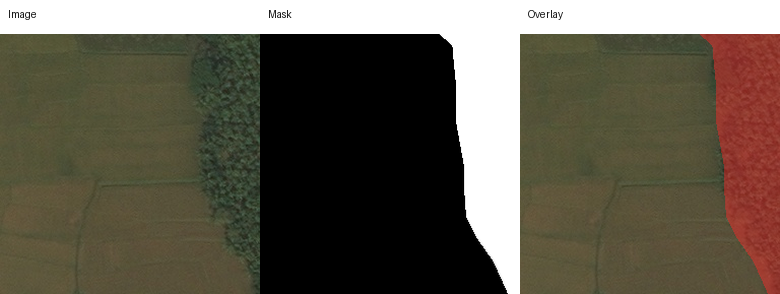
\includegraphics[width=\linewidth]{Figuras/forest_aerial_examplo.png}
}

\subfloat[]{
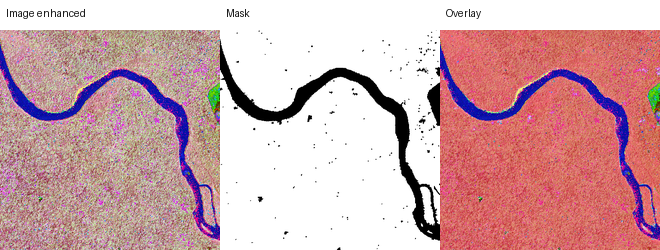
\includegraphics[width=\linewidth]{Figuras/amazon_atlantic_candidate_4.png}
}
\caption{(a) Representative example from the Forest Aerial Images dataset used for external cross-dataset evaluation. (b) Representative example from the Amazon/Atlantic Forest dataset used for external cross-dataset evaluation.}
\label{f4}
\end{figure}

\textcolor{red}{To assess cross-dataset transfer without adapting the trained weights, we evaluated the final checkpoints on two external datasets used exclusively for testing. The Forest Aerial Images dataset~\cite{quadeer2024augmentedforest} comprises 5,108 paired RGB images and corresponding binary forest masks, all of which were included in the evaluation. Since this local benchmark does not provide a predefined test partition, the complete paired set was treated as an independent external evaluation set and was not used at any stage of DeforTrack training or model selection. The native $256\times256$ RGB images match the U-Net input resolution. For YOLO and Mask R-CNN, the predicted masks were mapped back to the native mask dimensions prior to metric computation, whereas U-Net images and masks were evaluated directly at $256\times256$.}

\begin{table}[!t]
\color{red}
\centering
\caption{Top three models by IoU on each external forest/non-forest segmentation dataset.}
\label{t6}
\scriptsize
\resizebox{\columnwidth}{!}{%
\begin{tabular}{|c|c|c|c|c|c|}
\hline
\textbf{External dataset} & \textbf{Rank} & \textbf{Model} & \textbf{Images} & \textbf{IoU [\%]} & \textbf{Dice/F1 [\%]} \\
\hline
Forest Aerial Images~\cite{quadeer2024augmentedforest} &
1 & U-Net & 5,108 & \textbf{60.58} & \textbf{70.36} \\
\hline
Forest Aerial Images~\cite{quadeer2024augmentedforest} &
2 & Mask R-CNN R-101 DC5 3x & 5,108 & 60.13 & 68.05 \\
\hline
Forest Aerial Images~\cite{quadeer2024augmentedforest} &
3 & Mask R-CNN R-101 FPN 3x & 5,108 & 53.61 & 61.10 \\
\hline
Amazon/Atlantic Forest~\cite{bragagnolo2021amazon} &
1 & YOLOv11n & 599 & \textbf{47.96} & \textbf{58.59} \\
\hline
Amazon/Atlantic Forest~\cite{bragagnolo2021amazon} &
2 & YOLOv8s & 599 & 25.79 & 33.51 \\
\hline
Amazon/Atlantic Forest~\cite{bragagnolo2021amazon} &
3 & YOLOv8l & 599 & 7.52 & 10.68 \\
\hline
\end{tabular}%
}
\end{table}

\textcolor{red}{The Amazon/Atlantic Forest benchmark~\cite{bragagnolo2021amazon} contributed the 599 samples for which image--mask pairs were locally available. These samples were also used only for external testing, independently of the source dataset's original train/validation labels. The source images are $512\times512$ four-band Sentinel-2 Level-2A patches containing red, green, blue, and near-infrared bands. Because all DeforTrack models were trained on three-channel RGB input, only the red, green, and blue bands were retained and the near-infrared band was discarded. This is therefore both a dataset-domain and a sensor-domain transfer experiment, rather than a like-for-like RGB aerial comparison. The external labels were converted to the same binary convention used by DeforTrack (forest $=1$, non-forest $=0$). YOLO predictions were produced from internally resized $640\times640$ inputs and restored to the native $512\times512$ mask size for scoring, whereas the U-Net inputs and masks were resized to $256\times256$.}

\textcolor{red}{Table~\ref{t6} shows that external performance depends strongly on the visual and sensor characteristics of each dataset. On Forest Aerial Images, U-Net ranked first with $60.58~\%$ IoU and $70.36~\%$ Dice/F1, followed closely by Mask R-CNN R-101 DC5 3x with $60.13~\%$ IoU and then Mask R-CNN R-101 FPN 3x with $53.61~\%$. U-Net's result should not be interpreted as evidence of universally superior generalization: this dataset has the same native resolution as the U-Net input and contains comparatively broad, visually homogeneous forest regions, whereas downsampling DeforTrack from $640\times640$ to $256\times256$ can suppress narrow and fragmented boundaries. On the more dissimilar Sentinel-2 benchmark, YOLOv11n ranked first with $47.96~\%$ IoU, followed by YOLOv8s with $25.79~\%$ and YOLOv8l with $7.52~\%$. The large separation between first and second place, together with the low scores of the remaining models, exposes the severity of the sensor and domain shift instead of masking it behind the best result alone. Different class distributions and scene difficulty prevent direct ranking across datasets. These results demonstrate partial model-dependent transfer but do not establish geographic, biome-specific, or sensor-invariant generalization. Figure~\ref{f4} shows representative samples from both external benchmarks.}

\textcolor{red}{Table~\ref{t6} intentionally presents only the three highest-IoU checkpoints for each external dataset. Results for every evaluated checkpoint, including models outside the top three, are provided in machine-readable form under \texttt{results/cross\_dataset/}. All primary external results use the confidence and binarization thresholds fixed by the internal protocol; no threshold was optimized on either external dataset.}

\begin{figure}[!ht]
    \centering
    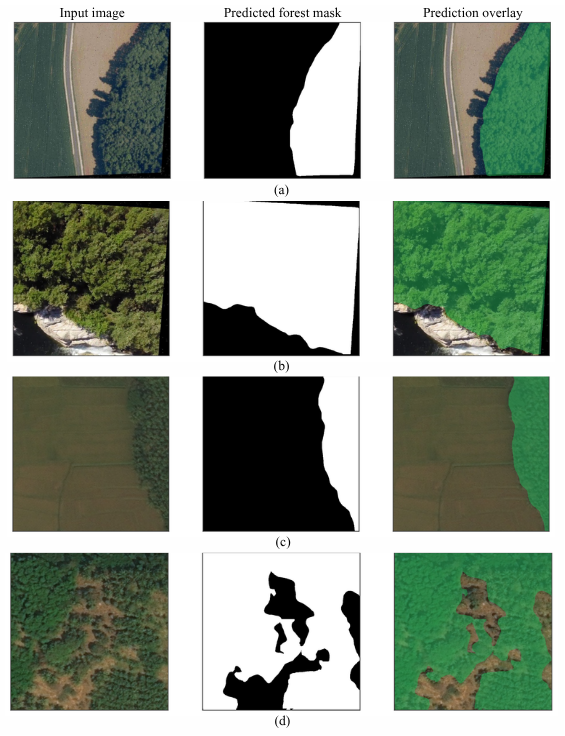
\includegraphics[width=\linewidth]{Figuras/F5.png}
    \caption{\small{Representative YOLOv8s segmentation results. DeforTrack scenarios: (a) vegetation–field boundary and (b) dense canopy. External images: (c) forest–field boundary and (d) mixed forest and open land-cover patterns.}}
    \label{f5}
\end{figure}

\begin{figure}[!ht]
    \centering
    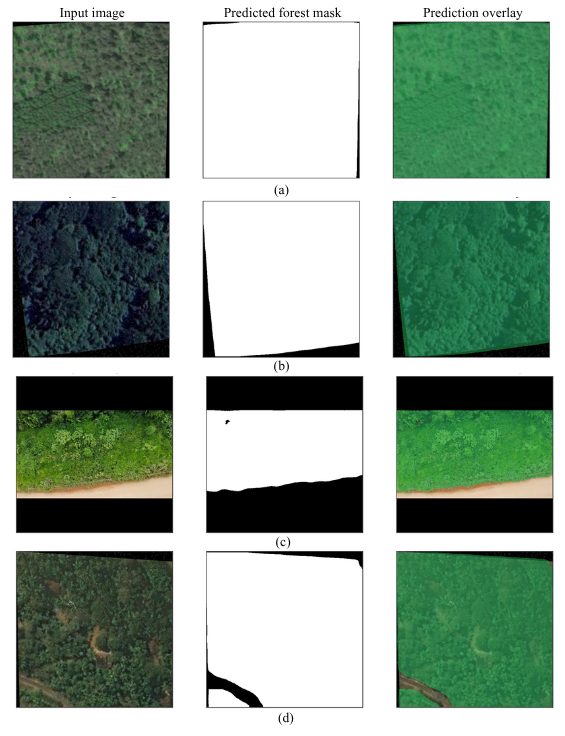
\includegraphics[width=\linewidth]{Figuras/F6.png}
    \caption{\small{Qualitative YOLOv8s segmentation result in different scenarios: (a) high forest cover, (b) continuous canopy, (c) forest boundary, and (d) fragmented canopy.}}
    \label{f6}
\end{figure}

\subsection{Qualitative Segmentation Examples}
\label{sec:qualitative_examples}

Qualitative examples were selected to illustrate the behavior of the YOLOv8s model under visually distinct forest segmentation scenarios. The examples include dense canopy, vegetation-field boundaries, and mixed land-cover patterns, covering both DeforTrack images and external RGB aerial imagery with visual characteristics similar to the proposed dataset. Figure~\ref{f5}(a) illustrates a vegetation-field boundary scenario, in which the model segments a compact forest fragment adjacent to agricultural land. Figure~\ref{f5}(b) shows a dense canopy scenario from DeforTrack, where the model predicts a large continuous forest region consistent with the homogeneous vegetation texture. Figures~\ref{f5}(c-d) show external RGB aerial examples, indicating that the model can transfer its learned forest-boundary representation to visually compatible imagery, although mixed land-cover scenes remain more challenging.

Additional qualitative examples are presented in Figure~\ref{f6}, following the same visual structure, showing the input image, the predicted forest mask, and the prediction overlay. They further illustrate model behavior under additional visual conditions, including high forest-cover regions, continuous canopy, forest boundaries, heterogeneous vegetation, and fragmented canopy patterns. Since complete image-level biome metadata is not available for all samples in the final exported dataset, these examples should be interpreted as visually distinct forest and land-cover scenarios rather than confirmed biome-specific samples.

\textcolor{red}{Across the visually simpler dense-canopy examples, the predicted masks remain largely continuous because color and texture are comparatively homogeneous. At vegetation--field transitions, the model generally follows the dominant canopy edge, but the decision becomes less stable where low vegetation, cultivated rows, exposed soil, or cast shadows interrupt that edge. Fragmented-canopy scenes are more demanding: small disconnected crowns may be omitted as false negatives, whereas dark non-forest patches or textured agricultural vegetation may be incorporated as false positives. The qualitative examples therefore support the aggregate ranking but also show why boundary-oriented scores remain substantially lower than region IoU and Dice/F1. They should be read as a scenario-level error analysis, not as evidence that performance is uniform across locations or biomes.}

\subsection{Limitations and Generalization Considerations}
\label{sec:limitations}

\textcolor{red}{Although the quantitative and qualitative results indicate that YOLO-based models achieved the best trade-off between segmentation accuracy and computational efficiency on the final test set, some limitations constrain their interpretation. Segmentation errors are more likely under shadows, strong illumination variation, low contrast, sparse or dry vegetation, and mixed land-cover patterns. The most difficult cases occur near visually ambiguous forest/non-forest transitions. Fragmented landscapes, exposed soil, agricultural fields, roads, shadows, and low vegetation density can resemble forest canopy or partially preserved vegetation, producing false positives. Conversely, sparse, low, or degraded forest can be omitted, producing false negatives. These failure modes show that aggregate metrics alone do not guarantee reliable behavior across all vegetation structures.}

\textcolor{red}{The most consequential dataset limitation is the absence of complete image-level geographic metadata in the final export. We audited all 14,648 exported JPEG images and their accompanying export structure. None contained EXIF metadata, GPS coordinates, or acquisition timestamps, and the export contained no authoritative sidecar fields assigning images to geographic regions, acquisition sources, or biomes. Filename searches also returned no explicit names of the six Brazilian biomes; filenames alone would in any case be insufficient as authoritative provenance. DeforTrack was designed for Brazilian deforestation monitoring and contains a predominance of Brazilian forest scenarios, but it also combines private and public sources from different regions. Consequently, a reliable retrospective assignment of every image to a Brazilian biome and an independently stratified spatial or temporal evaluation cannot be constructed from this export. The qualitative panels therefore represent distinct visual forest and land-cover scenarios, not confirmed examples of specific Brazilian biomes, and the current results must not be used to claim biome-specific performance.}

\textcolor{red}{The same export limitation affects item-level source and licensing traceability for the 5,344 images collected from public repositories. The Roboflow release metadata records a dataset-level CC BY 4.0 configuration, but the local export does not contain an authoritative per-image mapping to each upstream repository and license. Accordingly, dataset-level release metadata should not be interpreted as reconstructing or superseding upstream rights. A provenance manifest linking each public image to its source URL, original identifier, and reuse terms is required for a future fully traceable release; files whose upstream redistribution rights cannot be verified should be distributed only as identifiers, annotations, or acquisition scripts, as permitted by their original terms.}

\textcolor{red}{The current image-level split also does not demonstrate geographic or temporal independence. Splitting before augmentation reduces direct leakage from augmented derivatives, but no source-aware, region-wise, biome-aware, flight-wise, or date-wise grouping was available. Spatially close, visually similar, or temporally related samples may therefore share patterns across training, validation, and test partitions, potentially causing optimistic performance estimates. The 892-image test results are internally standardized across architectures, but they should be interpreted as performance under this partitioning protocol rather than as evidence of transfer to unseen locations or acquisition periods.}

\textcolor{red}{Future releases should preserve, whenever licensing and privacy permit, image-level provenance fields for source, geographic region or coordinates, Brazilian biome, sensor, flight or acquisition campaign, and acquisition date. Samples can then be grouped by those fields before partitioning to support source-aware, region-wise, biome-aware, and temporal holdout protocols. Such metadata and protocols are required before making robust claims about unseen regions, biomes, sensors, or land-cover change over time.}


\section{Conclusions}\label{sec:conclusions}

\textcolor{red}{This paper introduced DeforTrack, a large-scale, manually annotated dataset designed to advance deep learning-based forest segmentation and deforestation monitoring. Data collection produced an initial acquisition pool of 6,094 images from UAV surveys, imagery accessed through GEE, and public environmental repositories. After annotation and export curation, 6,074 source images are represented in the released partitions, which comprise 14,648 exported images after training-set augmentation. Beyond presenting the dataset itself, this work characterizes its acquisition categories, annotation quality, released forest-cover distribution, and current provenance limitations.}

\textcolor{red}{Standardized benchmarking of U-Net, Mask R-CNN, YOLOv8, and YOLOv11 on the same 892-image final test set showed that YOLO-based architectures provide the strongest accuracy--efficiency balance on the evaluated RTX 4060 Laptop GPU workstation. The framework complements segmentation metrics with platform-specific latency, throughput, memory, CPU, and GPU-energy measurements. These results support model selection for subsequent deployment studies, but do not by themselves demonstrate real-time operation or efficiency on an embedded device.}

% Although future work requires adopting source-aware, geographically stratified, biome-aware, and temporally independent validation protocols, the current dataset already provides a valuable benchmark for developing and comparing semantic segmentation methods for forest monitoring. 

\textcolor{red}{Although future work should adopt source-aware, geographically stratified, biome-aware, and temporally independent validation protocols, the current release provides a documented benchmark for developing and comparing semantic segmentation methods under the stated partitioning protocol. The public code, per-image outputs, manifests, and machine-readable result tables support computational reproduction of the reported analyses; they do not substitute for the missing source-, location-, time-, and license-level provenance required for broader claims of geographic generalization and fully traceable redistribution.}

%%%%%%%%%%%%%%%%%%%%%%%%%%%%%%%%%%%%%%%%%%

\vspace{6pt} 

%%%%%%%%%%%%%%%%%%%%%%%%%%%%%%%%%%%%%%%%%%
%% optional
%\supplementary{The following supporting information can be downloaded at:  \linksupplementary{s1}, Figure S1: title; Table S1: title; Video S1: title.}

% Only for journal Methods and Protocols:
% If you wish to submit a video article, please do so with any other supplementary material.
% \supplementary{The following supporting information can be downloaded at: \linksupplementary{s1}, Figure S1: title; Table S1: title; Video S1: title. A supporting video article is available at doi: link.}

% Only used for preprtints:
% \supplementary{The following supporting information can be downloaded at the website of this paper posted on \href{https://www.preprints.org/}{Preprints.org}.}

% Only for journal Hardware:
% If you wish to submit a video article, please do so with any other supplementary material.
% \supplementary{The following supporting information can be downloaded at: \linksupplementary{s1}, Figure S1: title; Table S1: title; Video S1: title.\vspace{6pt}\\
%\begin{tabularx}{\textwidth}{lll}
%\toprule
%\textbf{Name} & \textbf{Type} & \textbf{Description} \\
%\midrule
%S1 & Python script (.py) & Script of python source code used in XX \\
%S2 & Text (.txt) & Script of modelling code used to make Figure X \\
%S3 & Text (.txt) & Raw data from experiment X \\
%S4 & Video (.mp4) & Video demonstrating the hardware in use \\
%... & ... & ... \\
%\bottomrule
%\end{tabularx}
%}

%%%%%%%%%%%%%%%%%%%%%%%%%%%%%%%%%%%%%%%%%%
\authorcontributions{
Conceptualization, A. S. Careli, E. C. Vilas Boas, F. A. P. Figueiredo; 
methodology, A. S. Careli, L. P. Raimundo, G. G. Oliveira, E. C. Vilas Boas, F. A. P. Figueiredo; 
software, A. S. Careli, L. P. Raimundo, G. G. Oliveira; 
validation, A. S. Careli, L. P. Raimundo, G. G. Oliveira, F. A. P. Figueiredo; 
formal analysis, A. S. Careli, L. P. Raimundo, G. G. Oliveira, E. C. Vilas Boas, F. A. P. Figueiredo; 
investigation, A. S. Careli; 
resources, E. C. Vilas Boas, F. A. P. Figueiredo; 
data curation, A. S. Careli, L. P. Raimundo, G. G. Oliveira; 
writing---original draft preparation, A. S. Careli, E. C. Vilas Boas, F. A. P. Figueiredo; 
writing---review and editing, A. S. Careli, E. C. Vilas Boas, F. A. P. Figueiredo; 
visualization, A. S. Careli, E. C. Vilas Boas; 
supervision, E. C. Vilas Boas, F. A. P. Figueiredo; 
project administration, A. S. Careli, E. C. Vilas Boas, F. A. P. Figueiredo; 
funding acquisition, E. C. Vilas Boas, F. A. P. Figueiredo. All authors have read and agreed to the published version of the manuscript.}

\funding{This work has been partially funded by the xGMobile Project XGM-AFCCT-2026-8-27-1 with resources from EMBRAPII/MCTI (Grant 052/2023 PPI IoT/Manufatura 4.0), by CNPq (306199/2025-4), FAPEMIG (APQ-03162-24, APQ-04523-23, APQ-05305-23, PPE-00124-23, RED-00194-23), by FINEP (nº 1060/2 contract 01.25.0883.00), by RNP, with resources from MCTIC, Grant No. 01245.020548/2021-07, under the Brazil 6G project of the Radiocommunication Reference Center of Inatel, Brazil. We also acknowledge the support of ABRINT, MODIRUM/GESPI, and NIC.br.}

\informedconsent{Not applicable.}

\dataavailability{DeforTrack is publicly available to the research community~\url{https://universe.roboflow.com/alvaro-z5qmu/floresta-wgiln}} 

\conflictsofinterest{The authors declare no conflicts of interest.} 

%%%%%%%%%%%%%%%%%%%%%%%%%%%%%%%%%%%%%%%%%%
%% Optional

%% Only for journal Encyclopedia
%\entrylink{The Link to this entry published on the encyclopedia platform.}

\abbreviations{Abbreviations}{
The following abbreviations are used in this manuscript:
\\

\noindent 
\textcolor{red}{%
\begin{tabular}{@{}ll}
C4 & Fourth-stage convolutional backbone configuration\\
CI & Confidence Interval\\
CNN & Convolutional Neural Network\\
CPU & Central Processing Unit\\
DC5 & Dilated fifth-stage convolutional backbone configuration\\
FPN & Feature Pyramid Network\\
FPS & Frames per Second\\
GEE & Google Earth Engine\\
GPU & Graphics Processing Unit\\
IoU & Intersection over Union\\
mAP & mean Average Precision\\
NVML & NVIDIA Management Library\\
RAM & Random Access Memory\\
R-CNN & Region-based Convolutional Neural Network\\
RGB & Red, Green, and Blue\\
UAV & Unmanned Aerial Vehicle\\
YOLO & You Only Look Once\\
\end{tabular}%
}
}

%%%%%%%%%%%%%%%%%%%%%%%%%%%%%%%%%%%%%%%%%%
%% Optional
\appendixtitles{no} % Leave argument "no" if all appendix headings stay EMPTY (then no dot is printed after "Appendix A"). If the appendix sections contain a heading then change the argument to "yes".


%%%%%%%%%%%%%%%%%%%%%%%%%%%%%%%%%%%%%%%%%%
%\isPreprints{}{% This command is only used for ``preprints''.
\begin{adjustwidth}{-\extralength}{0cm}
%} % If the paper is ``preprints'', please uncomment this parenthesis.
%\printendnotes[custom] % Un-comment to print a list of endnotes


\reftitle{References}
\bibliography{refs.bib}

\PublishersNote{}
%\isPreprints{}{% This command is only used for ``preprints''.
\end{adjustwidth}
%} % If the paper is ``preprints'', please uncomment this parenthesis.
\end{document}
